\documentclass[11pt]{article}
\usepackage[T1]{fontenc}
\usepackage[utf8]{inputenc}
\usepackage{lmodern}
\usepackage[margin=1in]{geometry}
\usepackage{amsmath,amssymb,amsthm,mathtools,bm}
\usepackage{enumitem,booktabs,longtable,array,graphicx,xcolor}
\usepackage[numbers,sort&compress]{natbib}
\usepackage{microtype}
\usepackage{hyperref}
\usepackage[capitalise,noabbrev]{cleveref}
\hypersetup{colorlinks=true,linkcolor=blue!55!black,citecolor=blue!55!black,
  urlcolor=blue!55!black,pdfauthor={},
  pdftitle={Quadratic hulls on boxes: valid inequalities and semidefinite representability}}
\newcommand{\R}{\mathbb R}
\newcommand{\Q}{\mathbb Q}
\newcommand{\Sbb}{\mathbb S}
\newcommand{\Sn}[1]{\mathbb S^{#1}}
\DeclareMathOperator{\conv}{conv}
\DeclareMathOperator{\cone}{cone}
\DeclareMathOperator{\cl}{cl}
\DeclareMathOperator{\COP}{COP}
\DeclareMathOperator{\CP}{CP}
\DeclareMathOperator{\DNN}{DNN}
\DeclareMathOperator{\PSD}{PSD}
\DeclareMathOperator{\tr}{tr}
\DeclareMathOperator{\diag}{diag}
\DeclareMathOperator{\rank}{rank}
\newcommand{\inner}[2]{\left\langle #1,#2\right\rangle}
\newcommand{\norm}[1]{\left\lVert #1\right\rVert}
\newcommand{\abs}[1]{\left\lvert #1\right\rvert}
\newtheorem{theorem}{Theorem}[section]
\newtheorem{lemma}[theorem]{Lemma}
\newtheorem{proposition}[theorem]{Proposition}
\newtheorem{corollary}[theorem]{Corollary}
\theoremstyle{definition}
\newtheorem{definition}[theorem]{Definition}
\newtheorem{example}[theorem]{Example}
\newtheorem{conjecture}[theorem]{Conjecture}
\theoremstyle{remark}
\newtheorem{remark}[theorem]{Remark}

\title{Quadratic hulls on boxes:\\valid inequalities and semidefinite representability}
\author{}
\date{}
\setlength{\emergencystretch}{2em}
\begin{document}
\maketitle
\begin{abstract}
Convexifying the products of a few bounded continuous variables is a basic
step in relaxing a nonconvex quadratic program. We study which valid
inequalities are missing from existing local relaxations and when the exact
quadratic moment hull admits a finite semidefinite lift. An explicit rational
three-variable example separates a disjoint-support affine-square
certificate system, even when strengthened by the specified extended-triangle
second-order-cone inequalities. The example belongs to a family of valid
quadratic inequalities whose entire parameter range is enforced by one
positive-semidefinite block of order five and six nonnegative auxiliary
variables. We prove exposedness in the strict parameter region and extremality
in several boundary regimes. In three variables, we also classify every extreme
ray with positive square coefficients and positive values at all cube vertices:
apart from affine squares, these rays are generated by strict family members
up to cube symmetry. We establish a sharp
representability boundary: the full quadratic moment hull of a box has a
finite semidefinite lift in dimension at most three, but has none in dimension
at least four. The obstruction extends to polytopes with a simple vertex and
to sparse joint hulls whose positive-loop graph contains a $K_4$ minor;
components of at most three positive-loop vertices admit explicit lifts.
The nonrepresentability proofs transfer known results about completely
positive maps over real closed fields to these hulls. Archived computations
show that selective family blocks can match exact triple lifts on constructed
instances, while offering little improvement on most tested benchmark
instances.
\end{abstract}
\noindent\textbf{Keywords:} quadratic optimization; convex hull; semidefinite
relaxation; valid inequalities; spectrahedral shadow; sparse optimization.

\section{Introduction}\label{sec:introduction}

A quadratic objective on a box depends on the first and second moments of
its variables. Replacing the possible moment vectors by their convex hull
therefore gives an exact convex formulation. The difficulty is describing
that hull. Even a relaxation built from many valid inequalities can omit a
nonnegative quadratic with only three variables. Conversely, the existence
of an exact formulation in three variables does not imply that a larger
finite semidefinite formulation will be exact in four variables.

This paper studies these two issues through the cone of quadratics
nonnegative on $[0,1]^n$. We first identify a family of valid three-variable
inequalities that recent semidefinite and second-order-cone relaxations
miss. We then give an exact, small semidefinite formulation of that family.
The same cone provides the setting for a dimension threshold: the full
quadratic moment hull has a finite semidefinite lift precisely when
$n\le3$. The negative result also holds when positive surplus is allowed
on the diagonal moments. This variant is the appropriate joint hull for
objectives whose square coefficients are nonnegative.

The connection between the two parts is concrete. A nonnegative quadratic
is a valid linear inequality for the moment hull. A certificate system
describes a subcone of these quadratics, and its dual defines a relaxation.
The new family fills a proved gap in one such system. The representability
result determines where any finite semidefinite system, regardless of its
chosen certificates or auxiliary variables, must cease to be exact.

\subsection{Relation to prior work}

Standard box relaxations combine the Shor moment-matrix condition
\citep{Shor1987QuadraticOptimization} with McCormick inequalities for
bilinear products \citep{McCormick1976}. The continuous polynomial form
of the reformulation--linearization technique (RLT) provides a systematic
framework for linearizing products of bound inequalities
\citep{SheraliTuncbilek1992}.

Anstreicher and Burer gave exact completely positive descriptions of
quadratic moment hulls on low-dimensional polytopes
\citep{AnstreicherBurer2010}. Triangulating a polytope of dimension at most
three produces completely positive blocks of order at most four. At these
orders, complete positivity is equivalent to positive semidefiniteness
and entrywise nonnegativity \citep{Diananda1962,MaxfieldMinc1962}.
Thus the exact three-variable box hull already has a finite semidefinite
lift. We use that construction both as a mathematical reference and as an
exact local strengthening in the archived computational comparisons. We do
not propose a first exact formulation for this hull.

Burer and Dong developed recursive descriptions and separation methods
for the related box completely positive and copositive cones
\citep{BurerDong2013}. An exact separation procedure and a finite
semidefinite lift are different properties. Our impossibility theorem
concerns the latter; it does not prevent separation or other exact
optimization methods.

Recent work seeks formulations that exploit sparse objectives and small
local blocks. Khajavirad's disjoint-support construction uses sums of
affine squares weighted by products of box literals, with the affine
factor involving only variables absent from the weight
\citep{Khajavirad2026SparseBoxQP}. In three variables with positive square
coefficients, the resulting extended formulation consists of $27$
localizing matrices. Anstreicher and Puges strengthen the usual
three-variable inequalities using a trilinear auxiliary variable and
second-order-cone inequalities \citep{AnstreicherPuges2025ETRI}. We give a
single rational moment functional feasible for both systems, including all
coordinate complements and permutations of the latter inequalities, but
violating a nonnegative quadratic. This is a comparison against the
specified systems, rather than a claim about all possible SOS or SOC
relaxations.

Sign structure supplies an additional point of comparison.
Burer, Natarajan, and Willemsen prove exactness of a semidefinite
relaxation for submodular box quadratics in at most three variables
\citep{BurerNatarajanWillemsen2025}. Combined with cube symmetries, this
result settles the three-variable disjoint-support certificate question
for quadratics with nonnegative square coefficients whenever the product
of the three mixed coefficients is nonpositive.
The new inequalities occupy the remaining sign class. This restriction
helps explain why they require three variables and why two-variable
restrictions do not detect them.

Hildebrand's rank-one subtraction criterion for copositive matrices
\citep{Hildebrand2014MinimalZeros} supplies a further geometric tool.
Applied through the cube vertices, it implies that the zeros of a
non-square extreme quadratic must affinely span the box. We combine this
criterion with an explicit analysis of convex facet restrictions and a
classification of cube-edge contact graphs. Together with the submodular
duality argument, these steps classify every extreme ray with positive
square coefficients and no vertex zero. The subtraction criterion is
prior work; the facet analysis and the resulting box classification are
the developments proved here.

For the negative representability result, the essential external tool is
the characterization of spectrahedral shadows by preservation under
completely positive maps over real closed fields due to Bodirsky, Kummer,
and Thom \citep{BodirskyKummerThom2024}. Their construction uses the Horn
copositive matrix to exhibit an obstruction to semidefinite
representability. We transfer that obstruction to quadratics on a box by
using the constant monomial as one copositive coordinate and placing the
other four coordinates near a box vertex. The transfer rules out every
finite semidefinite lift, rather than only a doubly nonnegative
approximation. We also extend the argument to polytopes with a simple
vertex and to sparse positive-loop graphs containing a $K_4$ minor.
These conclusions use the existing preservation theorem; the application
to the box and the stated sparse hulls is the result proved here.

Nishijima proves that the copositive and completely positive cones over
any symmetric cone of rank at least five are not spectrahedral shadows
\citep[Theorem~3.2]{Nishijima2026}. The present paper uses the explicit
box embedding and graph reductions to reach the moment hulls studied here.

\subsection{Contributions and scope}

The paper makes the following contributions.

\begin{enumerate}[leftmargin=*,itemsep=5pt]
\item An exact rational certificate proves that the three-variable
disjoint-support system misses a quadratic with strictly positive square
coefficients.
The same certificate satisfies the switched SOC strengthening of
Anstreicher and Puges. A direct proof using five edge zeros explains the
failure without a numerical optimization argument
(\cref{family:counterexample-section}).

\item A parameter family generalizes this example. Its validity follows
from an explicit polynomial identity. In an open parameter region its
members generate exposed extreme rays of the nonnegative-quadratic cone
and admit no disjoint-support certificate. All inequalities in the larger
validity domain are enforced by one positive semidefinite block of order
five and six nonnegative scalars, using only first and second moments
(\cref{family:section}).

\item We establish the closedness and dual interpretation of the
disjoint-support cone, relate diagonal caps to the distinction between
the full and positive-loop hulls, and prove the sign restriction and
boundary extreme-ray results needed to state a precise three-variable
completeness question. We further classify every extreme ray with positive
square coefficients and positive values at all cube vertices, reducing
the remaining completeness question to vertex-zero rays
(\cref{sec:three}). The completeness question remains separate
from the validity and enforcement theorems.

\item We prove the sharp dimension threshold for finite semidefinite
lifts of the full box moment hull, the positive-loop hull, and their
dual cones. We prove a local geometric extension at simple vertices and
show that every proper face of the four-variable box hull nevertheless
has such a lift (\cref{repr:section}).

\item For sparse moment hulls, we prove a $K_4$-minor obstruction on the
positive-loop subgraph and construct finite lifts when every positive-loop
component has at most three vertices. The construction gives an explicit
size bound in terms of a tree decomposition after the component boundaries
are made cliques (\cref{graph:section}). Archived computations compare the
new inequalities with the named relaxations and exact local hulls, with
separate conclusions for constructed and benchmark instances
(\cref{comp:section}).
\end{enumerate}

To the best of our knowledge, the family and its order-five formulation,
the exact separating certificate against the two named recent systems,
the classification of three-variable extreme rays with positive square
coefficients and no vertex zero, and the
stated box and sparse-graph representability consequences have
not appeared in the prior work reviewed here. The proofs below specify
these claims independently of priority. In particular, neither the
classical order-four cone identity nor the existing three-variable
tetrahedral lift is a new result.

The practical use of the family is local convexification. Each selected
triple contributes a block with no trilinear or higher-order moment
variables, so the inequalities can strengthen a relaxation that already
shares first and second moments. The archived study contains constructed
instances where this formulation attains the bound of exact triple hulls
with fewer selected blocks. On the tested natural instances, the base
relaxations were often already exact, and the new family produced little
additional improvement. These findings support selective use of the
family; they do not establish a general speed advantage or a
branch-and-bound performance improvement.

\Cref{sec:setting} fixes the moment and coefficient conventions.
\Cref{family:counterexample-section,family:section,sec:three} develop the
three-variable inequalities and their geometry.
\Cref{repr:section,graph:section} treat finite representability.
\Cref{comp:section} presents the archived computational evidence.
The appendices contain the exact moment certificate, boundary calculations,
stationary-facet and contact-graph proofs, real closed field details, and
separation and comparison tools.

\section{Quadratic moments and certificate systems}\label{sec:setting}

\subsection{The full hull and the positive-loop hull}\label{set:cones}
Let $C_n=[0,1]^n$. We write a quadratic as
\begin{equation}\label{eq:set:quadratic}
 q(x)=q_0+\sum_{i=1}^n a_ix_i+\sum_{i=1}^n b_ix_i^2
                  +\sum_{1\le i<j\le n}c_{ij}x_ix_j.
\end{equation}
Thus $c_{ij}$ is the coefficient of the monomial $x_ix_j$, rather than an
off-diagonal entry of a symmetric matrix representing $q$. Define
\[
 \mathcal P_n=\{q:q(x)\ge0\text{ for every }x\in C_n\},\qquad
 \mathcal P_n^+=\{q\in\mathcal P_n:b_i\ge0\text{ for every }i\}.
\]
The corresponding moment sets are
\begin{equation}\label{eq:set:hulls}
 \mathcal Q_n=\conv\{(x,xx^\top):x\in C_n\},\qquad
 \mathcal H_n=\mathcal Q_n+
       \{(0,\diag(s)):s\in\R_+^n\}.
\end{equation}
The set $\mathcal Q_n$ is compact. The set $\mathcal H_n$ is closed because
it is the sum of a compact set and a closed cone. A point $(m,Y)$ in
$\mathcal Q_n$ records the first and second moments of a finite probability
law on the box. In $\mathcal H_n$, each diagonal second moment may also
contain nonnegative slack. We use the name \emph{positive-loop hull} for this
second set: a loop is the graph coordinate representing a square, and its
sign specifies the permitted direction of diagonal slack.

For a quadratic, its evaluation at moments is
\begin{equation}\label{eq:set:pairing}
 \mathcal L_{m,Y}(q)=q_0+\sum_i a_im_i+\sum_i b_iY_{ii}
                         +\sum_{i<j}c_{ij}Y_{ij}.
\end{equation}
Every $q\in\mathcal P_n$ gives a valid inequality $\mathcal L_{m,Y}(q)\ge0$ for
$\mathcal Q_n$. It is valid for $\mathcal H_n$ exactly when $q\in\mathcal P_n^+$.
Indeed, evaluating at $(x,xx^\top)$ gives $q(x)$, while adding diagonal
slack changes the value by $\sum_i b_is_i$. Conversely, finite-dimensional
separation shows that these valid inequalities describe the two closed
convex sets.

These are joint hulls of all recorded products. A lift of an epigraph for
one fixed objective need not describe the full moment hull. This distinction
will matter in the nonrepresentability results.

\subsection{Normalization and duality}\label{set:dual}
Taking cone duals requires retaining the constant coordinate. Let
\[
 \widehat{\mathcal Q}_n
   =\cone\{(1,x,xx^\top):x\in C_n\},\qquad
 \widehat{\mathcal H}_n
   =\widehat{\mathcal Q}_n+
       \{(0,0,\diag(s)):s\in\R_+^n\}.
\]
Both cones are closed. In the first cone, every coordinate is bounded in
absolute value by its mass coordinate, so a convergent sequence with mass
tending to zero has limit zero. The same argument in the second cone leaves
only the displayed diagonal slack when the mass tends to zero. For positive
mass, closure follows by rescaling to the compact set $\mathcal Q_n$ and
extracting a convergent slack vector.

Under the pairing obtained from \eqref{eq:set:pairing} by replacing $q_0$
with $tq_0$, their dual cones are $\mathcal P_n$ and $\mathcal P_n^+$,
respectively. Their mass-one slices are $\mathcal Q_n$ and $\mathcal H_n$.
The zero-mass slack in $\widehat{\mathcal H}_n$ cannot be discarded when
using homogeneous duality.

We call a set a \emph{spectrahedral shadow}, or equivalently a set with a
\emph{finite semidefinite lift}, if it can be written as
\begin{equation}\label{eq:set:shadow}
 \{y:\exists z,\ A_0+\textstyle\sum_i y_iA_i+\sum_j z_jB_j\succeq0\},
\end{equation}
possibly with additional affine equalities. Several PSD blocks are allowed,
since they can be combined in one block-diagonal matrix. The word ``finite''
places no polynomial bound on the number of auxiliaries or the block orders.
Consequently, failure of finite representability is stronger than failure
of a particular small relaxation. It is not a computational hardness theorem.

\subsection{The three-variable disjoint-support system}\label{set:disjoint}
For the remainder of the local certificate analysis, $n=3$. Let $W$ be
the ten-dimensional vector space of quadratics, including their constants.
Let $V$ be the twenty-dimensional span of the monomials $x^\alpha$ with
$\alpha\in\{0,1,2\}^3$ and at most one exponent equal to two. For disjoint
subsets $A,B\subseteq\{1,2,3\}$, put
\[
 w_{A,B}(x)=\prod_{i\in A}x_i\prod_{j\in B}(1-x_j),\qquad
 F_{A,B}=\{1,2,3\}\setminus(A\cup B).
\]
Let $v_F(x)$ list the constant one and the coordinates indexed by $F$.
Define the cone
\begin{equation}\label{eq:set:disjoint}
 \mathcal K_D=\left\{\sum_{A\cap B=\varnothing}
       w_{A,B}(x)v_{F_{A,B}}(x)^\top G_{A,B}v_{F_{A,B}}(x):
       G_{A,B}\succeq0\right\}\subseteq V,
 \qquad \mathcal D_3=\mathcal K_D\cap W.
\end{equation}
Each summand is nonnegative on the cube. The matrix representation permits
any finite sum of affine squares on the unused coordinates. The requirement
that the final sum belongs to $W$ imposes cancellation of all monomials of
degree greater than two; it must not be replaced by a degree restriction on
each summand. In particular, $\mathcal D_3\subseteq\mathcal P_3^+$: the coefficient
of $x_i^2$ comes only from a nonnegative diagonal entry of a block whose
unused coordinates include $i$.

The dual local relaxation consists of restrictions to $W$ of functionals
$\ell\in V^*$ satisfying
\begin{equation}\label{eq:set:localizing}
 \ell(1)=1,\qquad
 M_{A,B}(\ell):=
       \ell\bigl(w_{A,B}v_{F_{A,B}}v_{F_{A,B}}^\top\bigr)\succeq0
       \quad(A\cap B=\varnothing).
\end{equation}
Here $\ell$ acts entrywise on a polynomial matrix. Write $\mathcal R_D$ for the
resulting set of quadratic moment pairs $(m,Y)$, with
$m_i=\ell(x_i)$ and $Y_{ij}=\ell(x_ix_j)$. There are $27$ blocks:
eight of order one, twelve of order two, six of order three, and one of
order four. The higher moments in $V\setminus W$ are auxiliary coordinates.
They need not come from one probability law. Every point of $\mathcal H_3$
has such an extension; conversely, equality of the relaxation with that
hull is the substantive exactness question. \Cref{sec:three} proves the
closedness and extension statements needed to use this primal--dual
description without a hidden closure assumption.

\subsection{Diagonal caps and cube symmetries}\label{set:caps}
The full box hull satisfies the three inequalities
\begin{equation}\label{eq:set:caps}
 Y_{ii}\le m_i\quad(i=1,2,3),
\end{equation}
which are the moment forms of $x_i(1-x_i)\ge0$. We call them
\emph{diagonal caps}. They have negative square coefficients and are not
valid for the unbounded positive-loop hull. Thus a proposed description of
$\mathcal Q_3$ and a proposed description of $\mathcal H_3$ are different
statements, even when all other inequalities are the same.

\label{set:symmetry}
Coordinate permutations and complements $x_i\mapsto1-x_i$ preserve the
cube. They induce affine maps on normalized first and second moments and
linear maps on homogeneous moments. Complementing coordinate $i$, for
example, sends
\[
 m_i\mapsto1-m_i,\quad
 Y_{ii}\mapsto1-2m_i+Y_{ii},\quad
 Y_{ij}\mapsto m_j-Y_{ij}\quad(j\ne i),
\]
with simultaneous substitution when more than one coordinate is
complemented. These symmetries preserve $\mathcal Q_3$, $\mathcal H_3$,
and the disjoint-support certificate and moment systems. They provide the
different orientations of the inequality family constructed below.

\section{A gap in the disjoint-support relaxation}
\label{family:counterexample-section}

The disjoint-support construction includes an affine-square certificate on
every face of the cube. These certificates do not suffice for all nonnegative
quadratics, even when every square coefficient is strictly positive. The
following example gives both a geometric obstruction and an exact moment
certificate of the gap.

\begin{theorem}
\label{family:counterexample}
The quadratic
\begin{equation}
\label{family:example-polynomial}
p(x,y,z)=x^2+y^2+9z^2+6xy-12xz-12yz-x-y+9z+\tfrac14
\end{equation}
belongs to $\mathcal P_3^+$ but not to $\mathcal D_3$.
Its minimum on $C_3$ is zero, and its zero set consists of the five points
\begin{equation}
\label{family:five-zeros}
\begin{split}
a&=(\tfrac12,0,0),\qquad b=(0,\tfrac12,0),\\
c&=(1,0,\tfrac16),\qquad d=(0,1,\tfrac16),\qquad
e=(1,1,\tfrac56).
\end{split}
\end{equation}
\end{theorem}

\begin{figure}[htbp]
\centering
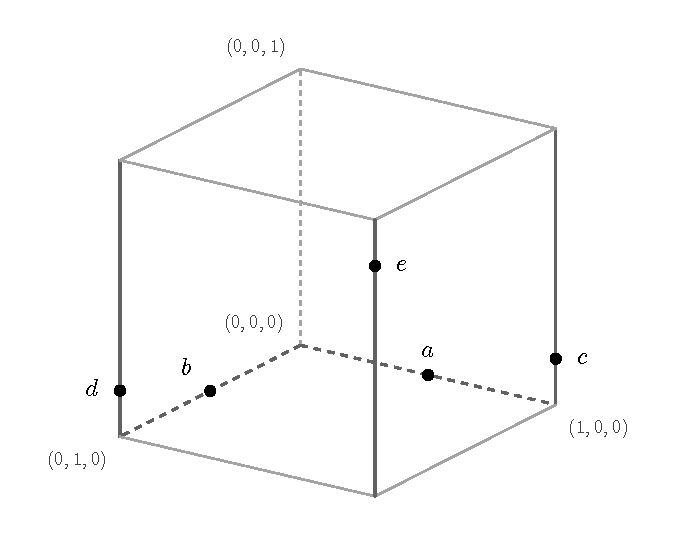
\includegraphics[width=0.60\linewidth]{figures/five-edge-zeros.pdf}
\caption{The five interior edge zeros of $p$ in \eqref{family:five-zeros}.
Darker edges contain zeros; dashed lines indicate rear cube edges.
These contacts explain the disjoint-support obstruction and determine
the exposed ray in \Cref{family:exposed}.}
\label{family:contact-figure}
\end{figure}

\begin{proof}
The polynomial identity
\begin{equation}
\label{family:example-identity}
\begin{split}
p={}&(xy+x+y-3z-\tfrac12)^2+6z(1-x)(1-y)\\
   &+3xy(1-x)+2xy(1-y)+x^2y(1-y)
\end{split}
\end{equation}
proves nonnegativity on the cube. Its square coefficients are $1,1,9$.
At a zero, the third and fourth terms imply either $xy=0$ or $x=y=1$.
If $y=0$, the second term implies $z=0$ or $x=1$; the square then gives
$a$ or $c$. The case $x=0$ gives $b$ or $d$. If $x=y=1$, the square gives
$e$. Each of these five points is indeed a zero.

Suppose that $p$ has a disjoint-support certificate. Since
$p(0,0,0)=1/4$, some individual term $w_{A,B}\ell^2$ is strictly positive
at the origin. Its weight must have $A=\varnothing$, and its affine factor
has the form
$\ell=\alpha+\beta x+\gamma y+\delta z$ with $\alpha\ne0$.
Every term in the certificate is nonnegative on the cube, so this term
vanishes at each point in \eqref{family:five-zeros}.

The weight is strictly positive at $a$ and $b$, for every possible $B$.
Thus $\beta=\gamma=-2\alpha$. The support restriction now excludes $x$
and $y$ from $B$, so $B\subseteq\{z\}$. The weight is consequently
strictly positive at $c$ and $e$. Vanishing at $c$ gives
$\delta=6\alpha$, whereas at $e$ the affine factor has value $2\alpha$.
This contradicts its required vanishing.
\end{proof}

The identity \eqref{family:example-identity} also identifies what the
disjoint construction omits. It uses a bilinear expression inside a square,
and a factor $y(1-y)$ whose two literals concern the same coordinate.
Neither is allowed in $\mathcal K_D$. The exclusion proof does not depend
on a degree truncation: in three variables all permitted generators already
have degree at most four, and all of them are included in $\mathcal K_D$.

The five zeros in \Cref{family:contact-figure} explain the obstruction.
An interior zero on an edge forces
every certificate term whose weight is positive there to vanish through
its affine factor. For a term positive at the origin, the first two zeros
force both $x$ and $y$ to occur in that factor. The remaining zeros then
impose inconsistent affine equations. This argument concerns the support
restriction, rather than the size of a chosen semidefinite block.

\begin{proposition}[Exact moment gap]
\label{family:gap}
There is a linear functional $\Lambda$ on $V$, with $\Lambda(1)=1$, such
that all $27$ disjoint localizing matrices are positive definite and
\begin{equation}
\label{family:gap-value}
\Lambda(p)=-\tfrac1{40}.
\end{equation}
Its quadratic moments also satisfy $Y_{ii}<m_i$ for all three coordinates.
In particular, $p\notin\cl(\mathcal D_3)$, and every feasible lower bound
in the certificate problem
\[
\sup\{\gamma:p-\gamma\in\mathcal D_3\}
\]
is at most $-1/40$, although $\min_{C_3}p=0$.
\end{proposition}

\begin{proof}
Use the rational moments in \cref{family:moment-table}. Their localizing
matrices and positive leading determinants are given in
\cref{family:localizing-tables}. Since
$\Lambda(w_{A,B}\ell^2)$ is the quadratic form of the corresponding
positive definite matrix, $\Lambda$ is nonnegative on $\mathcal K_D$.
Substitution in \eqref{family:example-polynomial} gives
\eqref{family:gap-value}. Continuity therefore separates $p$ from
$\cl(\mathcal D_3)$ as well as from $\mathcal D_3$.
The diagonal upper-bound slacks are
\[
m_x-Y_{xx}=m_y-Y_{yy}=\frac{649}{10000},\qquad
m_z-Y_{zz}=\frac{696}{10000}.
\]
If $p-\gamma\in\mathcal D_3$, applying $\Lambda$ gives
$-1/40-\gamma\ge0$.
\end{proof}

This gap is not confined to quadratics with zeros. The polynomial
$p+1/80$ is at least $1/80$ throughout the cube, while
$\Lambda(p+1/80)=-1/80$. Thus even strict positivity does not make these
disjoint certificates complete.

\subsection{Comparison with two recent relaxations}
\label{family:comparison-subsection}

For three positive loops, the matrices in the disjoint-support system are
exactly the $27$ matrices in equation~(17) of
\citet{Khajavirad2026SparseBoxQP}. Their orders are $4,3,2,1$, with respective
multiplicities $1,6,12,8$. Consequently,
\cref{family:gap} gives a negative answer to the three-variable exactness
question for that system. This comparison uses the displayed matrices;
it does not require a convention about the degree of the SOS certificate.

The same functional satisfies the second-order-cone strengthening of the
extended triangle inequalities in \citet{AnstreicherPuges2025ETRI}.
Let $t=\Lambda(xyz)$. For distinct indices $i,j,k$, its two types of SOC
inequalities are
\begin{equation}
\label{family:ap-soc}
t^2\le Y_{ii}Y_{jk},\qquad
(Y_{ij}+t)^2\le Y_{ii}(Y_{jj}+3Y_{jk}),
\end{equation}
together with their coordinate permutations and complements. Their
trilinear RLT inequalities are the eight nonnegative scalar localizing
blocks. \Cref{family:ap-certificate} verifies all $24$ instances of the
first inequality and all $48$ instances of the second, with strictly
positive right-hand factors. The base moment matrix is positive definite,
and the separate diagonal upper bounds hold by \cref{family:gap}.
The nonnegative scalar blocks imply the off-diagonal RLT and ordinary
triangle inequalities; the SOC inequalities imply the three extended
triangle families by Lemmas~4--5 of \citet{AnstreicherPuges2025ETRI}.

It follows that intersecting either named relaxation with $p\ge0$ is a
strict strengthening. The family introduced next gives a compact way to
enforce this inequality and its parameter variations. This conclusion
does not assert that one family block dominates either relaxation on its
own. The established exact tetrahedral description of the three-variable
hull already implies $p\ge0$ \citep{AnstreicherBurer2010}.

\section{A valid family and its compact semidefinite formulation}
\label{family:section}

The example in \cref{family:counterexample} belongs to a parameter family
with the same five-edge geometry. The validity domain is larger than the
domain with five interior contacts. Retaining that larger domain is what
makes exact enforcement by a small semidefinite formulation possible.

For $h\in\R$ and $d_1,d_2,d_3,k\ge0$, set
$L=h-d_1x-d_2y+d_3z$ and $D=d_1+d_2-h$, and define
\begin{equation}
\label{family:definition}
q_{h,d,k}=L^2+2d_3kz(1-x-y)+k(2D+k)xy.
\end{equation}
In particular, $h$ is unrestricted in sign. Let $\mathcal F$ denote the
set of these polynomials, and let $\cone(\mathcal F)$ denote its conic
hull. Scaling all five parameters by $\alpha\ge0$ scales the polynomial
by $\alpha^2$.

\begin{theorem}[Validity]
\label{family:valid}
Every member of $\mathcal F$ belongs to $\mathcal P_3^+$. Hence every
inequality $\mathcal L_{m,Y}(q_{h,d,k})\ge0$ is valid on both
$\mathcal Q_3$ and $\mathcal H_3$.
\end{theorem}

\begin{proof}
The following polynomial identity holds for all real parameters:
\begin{equation}
\label{family:identity}
\begin{split}
q_{h,d,k}={}&(L-kxy)^2+2d_3kz(1-x)(1-y)\\
 &+k(2d_1+k)xy(1-x)+2kd_2xy(1-y)
   +k^2x^2y(1-y).
\end{split}
\end{equation}
To check it, expand the square and collect the remaining terms as
$2kxyL+2d_3kz(1-x-y)+k(2D+k)xy-k^2x^2y^2$.
After substituting $L$ and $D$, this is precisely the sum of the four
remaining terms in \eqref{family:identity}.
Each term on the right is nonnegative on $C_3$ under the stated parameter
restrictions. No sign condition on $h$ is used. The square coefficients
are $d_i^2$, so at an atom with diagonal surplus $s_i\ge0$ the evaluated
inequality has value
\[
q_{h,d,k}(x)+\sum_{i=1}^3d_i^2s_i\ge0.
\]
Convexity gives validity on $\mathcal Q_3$ and $\mathcal H_3$.
\end{proof}

Zero parameters are included in this result. For example, $k=0$ gives an
affine square, which already has a disjoint-support certificate. The
following theorem concerns the strict parameter region where the family
has five interior edge zeros.

\begin{theorem}[Exposed rays missed by disjoint certificates]
\label{family:exposed}
Assume
\begin{equation}
\label{family:strict-region}
h,d_1,d_2,d_3,k>0,\qquad h<\min\{d_1,d_2\},\qquad D+k<d_3.
\end{equation}
Then $q_{h,d,k}$ has exactly the five zeros
\begin{equation}
\label{family:contacts}
\begin{split}
a&=(h/d_1,0,0),\qquad b=(0,h/d_2,0),\\
c&=(1,0,(d_1-h)/d_3),\qquad
d=(0,1,(d_2-h)/d_3),\\
e&=(1,1,(D+k)/d_3).
\end{split}
\end{equation}
They lie in the relative interiors of their respective edges.
The ray $\R_+q_{h,d,k}$ is exposed in $\mathcal P_3$, and
$q_{h,d,k}\notin\mathcal D_3$.
\end{theorem}

\begin{proof}
The strict inequalities place each displayed zero in its edge interior.
The third and fourth terms of \eqref{family:identity} force any zero to
satisfy $xy=0$ or $x=y=1$. If $y=0$, the second term forces $z=0$ or
$x=1$; the square then gives $a$ or $c$. The case $x=0$ gives $b$ or $d$.
When $x=y=1$, the square gives $e$. Conversely all five points are zeros.

For exposedness, suppose that $r\in\mathcal P_3$ vanishes at these five
points. Write its coefficients in the convention of \cref{set:cones}:
\[
r=r_0+a_1x+a_2y+a_3z+b_1x^2+b_2y^2+b_3z^2
  +c_{12}xy+c_{13}xz+c_{23}yz.
\]
A univariate quadratic nonnegative on an interval and zero in its
interior is a nonnegative multiple of the square centered at that zero;
this includes the identically zero polynomial. Therefore
\[
r(x,0,0)=b_1(x-h/d_1)^2,\qquad
r(0,y,0)=b_2(y-h/d_2)^2,
\]
with $b_1,b_2\ge0$. Comparing constants shows that for some $\lambda\ge0$,
\begin{equation}
\label{family:contact-bottom}
b_1=\lambda d_1^2,\quad b_2=\lambda d_2^2,\quad
r_0=\lambda h^2,\quad
a_1=-2\lambda hd_1,\quad a_2=-2\lambda hd_2.
\end{equation}
The vertical restriction through $c$ is
$b_3(z-(d_1-h)/d_3)^2$. Evaluating at $z=0$ and using
$d_1-h>0$ gives $b_3=\lambda d_3^2$.
Vanishing of the three vertical derivatives at $c,d,e$ gives
\begin{align*}
a_3+c_{13}&=-2\lambda d_3(d_1-h),\\
a_3+c_{23}&=-2\lambda d_3(d_2-h),\\
a_3+c_{13}+c_{23}&=-2\lambda d_3(D+k).
\end{align*}
Solving yields
\begin{equation}
\label{family:contact-mixed}
a_3=2\lambda d_3(h+k),\qquad
c_{13}=-2\lambda d_3(d_1+k),\qquad
c_{23}=-2\lambda d_3(d_2+k).
\end{equation}
Finally, the restriction through $e$ gives
$r(1,1,0)=\lambda(D+k)^2$, and hence
\[
c_{12}=\lambda\bigl(2d_1d_2+k(2D+k)\bigr).
\]
Every coefficient of $r$ is now $\lambda$ times that of $q_{h,d,k}$.
The conclusion also holds when $\lambda=0$, in which case all coefficients
vanish. The functional
\[
r\longmapsto r(a)+r(b)+r(c)+r(d)+r(e)
\]
is nonnegative on $\mathcal P_3$ and has zero face exactly
$\R_+q_{h,d,k}$. It therefore exposes this ray.

For disjoint-certificate exclusion, use a term positive at the origin,
as in \cref{family:counterexample}. Write its affine factor as
$\alpha+\beta x+\gamma y+\delta z$, with $\alpha\ne0$ and
$A=\varnothing$. Its weight is positive at $a$ and $b$, so
$\beta=-\alpha d_1/h$ and $\gamma=-\alpha d_2/h$.
These nonzero coefficients force $B\subseteq\{z\}$. The weight is then
positive at $c$ and $e$. The zero at $c$ gives
$\delta=\alpha d_3/h$, but the affine factor has value $\alpha k/h\ne0$
at $e$, a contradiction.
\end{proof}

The exposed-ray conclusion is stronger than validity. A member in
\eqref{family:strict-region} cannot be decomposed into nonproportional
nonnegative quadratics. Its full mixed coefficients satisfy
$c_{12}>0$, $c_{13}<0$, and $c_{23}<0$. Their product is positive, which
agrees with the sign restriction in \cref{three:sign}.
For $(h,d_1,d_2,d_3,k)=(1/2,1,1,3,1)$, this theorem gives the polynomial
and zeros of \cref{family:counterexample}.

\subsection{Exact enforcement of all family inequalities}
\label{family:enforcement-subsection}

Let $\ell$ be a functional on quadratics, not necessarily a valid moment
functional. Write
$\ell(1)=t$, $\ell(x_i)=m_i$, and $\ell(x_ix_j)=Y_{ij}$, and form
\begin{equation}
\label{family:b-B}
b=\begin{pmatrix}-m_x\\-m_y\\m_z\\-Y_{xy}\end{pmatrix},\qquad
B=\begin{pmatrix}
Y_{xx}&Y_{xy}&-Y_{xz}&Y_{xy}\\
Y_{xy}&Y_{yy}&-Y_{yz}&Y_{xy}\\
-Y_{xz}&-Y_{yz}&Y_{zz}&m_z-Y_{xz}-Y_{yz}\\
Y_{xy}&Y_{xy}&m_z-Y_{xz}-Y_{yz}&Y_{xy}
\end{pmatrix}.
\end{equation}
Both depend linearly on the retained first and second moments.

\begin{theorem}[One order-five block and six auxiliaries]
\label{family:lmi}
For arbitrary $t,m,Y$, the inequalities
\[
\ell(q_{h,d,k})\ge0\qquad
(h\in\R,\ d_1,d_2,d_3,k\ge0)
\]
hold if and only if there is a symmetric matrix $N\in\Sbb^4$ satisfying
\begin{equation}
\label{family:homogeneous-lmi}
N_{ii}=0,\quad N_{ij}\ge0\ (i<j),\qquad
\begin{pmatrix}t&b^T\\ b&B-N\end{pmatrix}\succeq0.
\end{equation}
In particular, at $t=1$ they hold if and only if
$B-bb^T\in\COP_4$. The formulation uses one affine positive semidefinite
block of order five, six scalar nonnegative variables, and no moments of
degree greater than two.
\end{theorem}

\begin{proof}
Put $v=(d_1,d_2,d_3,k)^T$. Expanding
\eqref{family:definition} gives
\begin{equation}
\label{family:parameter-quadratic}
\ell(q_{h,d,k})=t h^2+2h b^Tv+v^TBv.
\end{equation}
At $v=0$, nonnegativity for every $h$ requires $t\ge0$.
If $t>0$, minimization over the unrestricted scalar $h$ gives
\[
\min_{h\in\R}\ell(q_{h,d,k})
  =v^T\bigl(B-t^{-1}bb^T\bigr)v,
\qquad h=-t^{-1}b^Tv.
\]
Thus the inequalities are equivalent to
$B-t^{-1}bb^T\in\COP_4$.

We use the classical order-four identity
\begin{equation}
\label{family:cop4}
\COP_4=\Sbb^4_++\mathcal N_4,
\qquad
\CP_4=\DNN_4,
\end{equation}
where $\mathcal N_4$ is the cone of symmetric entrywise nonnegative
matrices \citep{Diananda1962,MaxfieldMinc1962}.
It gives an exact decomposition
$B-t^{-1}bb^T=P+N$, with $P\succeq0$ and $N\ge0$ entrywise.
Moving the diagonal part of $N$ into $P$ permits $N$ to have zero diagonal.
The Schur complement of $t>0$ gives
\eqref{family:homogeneous-lmi}, and proves the converse as well.

If $t=0$, the expression in \eqref{family:parameter-quadratic} is
nonnegative for every real $h$ only if $b^Tv=0$ for all $v\ge0$,
or equivalently $b=0$. The remaining condition is $B\in\COP_4$.
By \eqref{family:cop4}, this again is exactly
\eqref{family:homogeneous-lmi}. Conversely, a positive semidefinite block
with zero top-left entry has $b=0$, so no additional case is needed.
This also covers the zero functional and all parameter degeneracies.
\end{proof}

The unrestricted sign of $h$ is essential to this proof. Requiring
$h\ge0$ would generally prevent elimination at $h=-b^Tv$ and would
produce a different condition. The nonnegative matrix $N$ is also
essential: setting $N=0$ can exclude valid cube moments. At the genuine
cube atom $(x,y,z)=(1/2,1/2,0)$, the matrix $B-bb^T$ has a zero first
diagonal entry but entry $(1,4)$ equal to $1/8$, so it is not positive
semidefinite. All family inequalities are nevertheless valid there.
The theorem is an SDP lift with auxiliary variables; it does not claim
an unlifted LMI or minimality of the stated lift size.

\subsection{Separation and extraction of a cut}
\label{family:separation-subsection}

At a normalized candidate moment point, let $A=B-bb^T$. The formulation
in \cref{family:lmi} can be tested as a feasibility SDP. Its equivalent
separation problem is
\begin{equation}
\label{family:separation-sdp}
\mu=\min\{\langle A,W\rangle: W\succeq0,\ W\ge0
             \text{ entrywise},\ \operatorname{tr}W=1\}.
\end{equation}

\begin{proposition}
\label{family:separation}
Problem \eqref{family:separation-sdp} has an attained optimum, and
\begin{equation}
\label{family:rankone-separation}
\mu=\min\{v^TAv:v\ge0,\ \|v\|_2=1\}.
\end{equation}
Thus $\mu<0$ if and only if some family inequality is violated.
A nonnegative vector $v$ with $v^TAv<0$, together with $h=-b^Tv$,
gives such an inequality.
\end{proposition}

\begin{proof}
The feasible set in \eqref{family:separation-sdp} is nonempty and compact.
For example, $(I+\mathbf1\mathbf1^T)/8$ is positive definite, strictly
positive entrywise, and has trace one. By $\DNN_4=\CP_4$, every feasible
$W$ has a finite decomposition $W=\sum_r u_ru_r^T$, with $u_r\ge0$.
Its trace condition gives $\sum_r\|u_r\|_2^2=1$. Discarding zero terms,
its objective is the convex combination
\[
\langle A,W\rangle
=\sum_r\|u_r\|_2^2
 \left(\frac{u_r}{\|u_r\|_2}\right)^T
 A\left(\frac{u_r}{\|u_r\|_2}\right).
\]
Conversely each normalized nonnegative rank-one matrix is feasible.
This proves \eqref{family:rankone-separation}; the last statement follows
from \eqref{family:parameter-quadratic} at $t=1$.
\end{proof}

A rank-one optimum exists, but an SDP solver need not return it.
A negative objective matrix is an aggregate certificate. Extracting
an individual cut from that matrix requires a completely positive
factorization, after which at least one factor has negative quadratic
value, or a separate search for a nonnegative vector. An exact
alternative using the $15$ nonempty coordinate supports is given in
\cref{comp:family-separation}. These statements concern exact arithmetic;
a numerical implementation must certify its proposed violation.

For the rational point in \cref{family:gap}, the parameters
$h=1/2$ and $v=(1,1,3,1)^T$ give $-1/40$. Keeping this $v$ fixed and
optimizing $h$ gives
\[
h=\frac{2361}{5000},\qquad
\ell(q_{h,d,k})=-\frac{644321}{25000000}.
\]
Hence the family block cuts off the point and strictly strengthens
each relaxation compared in \cref{family:comparison-subsection} when
added to that relaxation.

\subsection{Symmetry and selective use on larger problems}
\label{family:symmetries}

Coordinate permutations and complements preserve $C_3$, and therefore
preserve validity of the family. Their affine action on first and
second moments is given in \cref{set:symmetry}.
The diagonal surplus at an atom is unchanged, so the same transformations
preserve validity on $\mathcal H_3$ as well as on $\mathcal Q_3$.
Swapping $x$ and $y$ merely exchanges $d_1$ and $d_2$. Thus all symmetry
copies can be imposed using at most $24$ blocks: three choices of the
distinguished coordinate and eight complement patterns.

For a sparse quadratic model, one may add a family block on a selected
triple whose three edge moments are present. If an edge moment is absent,
introducing it is a further modeling choice. One may instead generate
individual inequalities by separation. The results above prove validity,
exact enforcement of the selected family, and strict improvement for
specified relaxation points. Completeness after every symmetry copy has
been included is the question examined in the next section.

\section{Structure of the three-variable cone}\label{sec:three}

The family in \Cref{family:definition} supplies inequalities missing from the
disjoint-support system. We now identify the part of the nonnegative
quadratic cone in which such inequalities can be needed. The argument also
separates two questions that a hull description must answer: whether the
diagonal caps have been imposed, and whether all inequalities with
nonnegative square coefficients have been found.

\subsection{Closedness and exact extension duality}

The higher-degree cancellations in \eqref{eq:set:disjoint} do not cause a
closure problem. This fact will let us use zero sets to exclude membership
in $\mathcal D_3$ without a separate limiting argument.

\begin{lemma}\label{three:closed}
The cones $\mathcal K_D$ and $\mathcal D_3$ are closed. The quadratic
\[
 q_*(x)=8+4(x_1^2+x_2^2+x_3^2)
\]
belongs to $W\cap\operatorname{int}\mathcal K_D$.
\end{lemma}
\begin{proof}
For a weight $w=w_{A,B}$ and its free coordinates $F$, let
\[
 H_w=\int_{C_3}w(x)v_F(x)v_F(x)^\top\,dx.
\]
This matrix is positive definite: the weight is positive in the interior
of the cube, and a nonzero affine function cannot vanish there. If a
sequence of polynomials in $\mathcal K_D$ converges in coefficients, choose a PSD
Gram matrix $G_{j,w}$ for each weight in each polynomial. Their integrals
are
\[
 \sum_w\tr(H_wG_{j,w}).
\]
These sums are bounded, and every summand is nonnegative. Since
$\tr(H_wG_{j,w})\ge\lambda_{\min}(H_w)\tr(G_{j,w})$, each sequence of Gram
matrices is bounded. A subsequence converges simultaneously in all $27$
blocks to PSD matrices representing the limiting polynomial. Thus $\mathcal K_D$
is closed, and so is its intersection with $W$.

Taking $G_w=I$ in every block gives
\[
 \sum_{A\cap B=\varnothing}w_{A,B}
       \left(1+\sum_{i\in F_{A,B}}x_i^2\right)
       =8+4\sum_i x_i^2.
\]
The linear map from the Gram blocks to $V$ is onto. Indeed, each monomial
in $V$ is a generator: use a constant square for a square-free monomial,
and use $x_i^2$ as the square when its exponent is two. The image of the
interior point consisting of identity Gram matrices is therefore an
interior point of $\mathcal K_D$.
\end{proof}

\begin{proposition}\label{three:extension}
Every linear functional on $W$ that is nonnegative on $\mathcal D_3$ has an
extension to $V$ that is nonnegative on $\mathcal K_D$. The moment relaxation $\mathcal R_D$
is closed, and, for a quadratic $q$,
\begin{equation}\label{eq:three:duality}
 \mathcal L_{m,Y}(q)\ge0\quad\hbox{for every }(m,Y)\in \mathcal R_D
 \quad\Longleftrightarrow\quad q\in \mathcal D_3.
\end{equation}
\end{proposition}
\begin{proof}
Let $T:V^*\to W^*$ be restriction. Because $q_*\in\operatorname{int}\mathcal K_D$,
there is an $\epsilon>0$ such that $q_*+\epsilon u\in \mathcal K_D$ whenever
$\norm{u}\le1$. Hence every $\ell\in \mathcal K_D^*$ satisfies
$\epsilon\norm{\ell}\le\ell(q_*)$. A convergent sequence $T\ell_j$ with
$\ell_j\in \mathcal K_D^*$ has bounded $\ell_j(q_*)$, and therefore a convergent
subsequence of extensions. Consequently $T(\mathcal K_D^*)$ is closed. Its dual is
$\mathcal K_D\cap W=\mathcal D_3$, so the bipolar theorem gives
$T(\mathcal K_D^*)=\mathcal D_3^*$. This proves the extension statement and the closedness of
the mass-one slice $\mathcal R_D$.

To account for normalization in \eqref{eq:three:duality}, note that
$\ell(1)\ge0$ for $\ell\in \mathcal K_D^*$. Positive-mass functionals can be
normalized. If $\ell(1)=0$, add $t$ times evaluation at any cube point,
normalize, and then let $t\downarrow0$. Nonnegativity on the mass-one
slice therefore implies nonnegativity on the entire cone $\mathcal K_D^*$, which
is equivalent to membership in $\mathcal K_D\cap W$.
\end{proof}

The same proof applies to the disjoint-support construction in two
variables. We write $\mathcal D_2$ and $\mathcal R_{D,2}$ for its quadratic cone and moment
relaxation.

\subsection{Diagonal caps and coordinate rounding}

For a coordinate $i$, define the linear map
\begin{equation}\label{eq:three:rounding}
 \rho_i f(x)=(1-x_i)f(x)|_{x_i=0}+x_if(x)|_{x_i=1}.
\end{equation}
For a probability law, composing its moment functional with $\rho_i$
replaces coordinate $i$, conditionally on the original point, by a
Bernoulli variable with the same mean. It keeps first moments and mixed
second moments, and sets the diagonal second moment to the first moment.

\begin{proposition}\label{three:caps}
For every $n$,
\begin{align}
 \mathcal P_n&=\mathcal P_n^+
       +\cone\{x_i(1-x_i):1\le i\le n\},\label{eq:three:cap-cone}\\
 \mathcal Q_n&=\mathcal H_n\cap
       \{(m,Y):Y_{ii}\le m_i\text{ for every }i\}.
       \label{eq:three:cap-hull}
\end{align}
In \eqref{eq:three:cap-cone}, the positive-square-coefficient component can
be chosen to have exactly the same mixed coefficients as the original
quadratic.
\end{proposition}
\begin{proof}
If the coefficient $b_i$ of $x_i^2$ is negative, then
\[
 \rho_iq=q+b_ix_i(1-x_i).
\]
The right side is nonnegative on the cube because it interpolates the
two nonnegative restrictions of $q$. Its $x_i^2$ coefficient is zero,
and no other square or mixed coefficient changes. Applying this operation
to every negative $b_i$ gives
\[
 q=q^++\sum_{b_i<0}(-b_i)x_i(1-x_i),\qquad q^+\in\mathcal P_n^+.
\]
The reverse inclusion is immediate.

For the hull statement, write a point of the right side as a true moment
point plus nonnegative diagonal slack. Take a finite probability law for
the true moment point. Rounding coordinate $i$ changes only its diagonal
moment, from its original value to $m_i$. A mixture of the original and
rounded laws realizes any value in this interval. Thus the assumed cap
allows us to match the prescribed $Y_{ii}$. Treating the coordinates in
turn changes no previously matched moment. This proves membership in
$\mathcal Q_n$. The other inclusion follows from $x_i^2\le x_i$ on the
cube.
\end{proof}

The disjoint-support relaxation has the same rounding property even when
its higher moments do not come from a probability law.

\begin{lemma}\label{three:rounding}
The map $\rho_i$ preserves $V$ and maps $\mathcal K_D$ into $\mathcal K_D$. If
$(m,Y)\in \mathcal R_D$, then both the point obtained by replacing $Y_{ii}$ by
$m_i$ and the point $(m,Y+tE_{ii})$, for $t\ge0$, belong to $\mathcal R_D$.
Consequently,
\begin{equation}\label{eq:three:round-slack}
 \mathcal R_D=\bigl(\mathcal R_D\cap\{Y_{ii}\le m_i\text{ for every }i\}\bigr)
       +\{(0,\diag(s)):s\ge0\}.
\end{equation}
\end{lemma}
\begin{proof}
On monomials in $V$, $\rho_i$ replaces $x_i^2$ by $x_i$ and fixes the
others. For a generator $w_{A,B}L^2$, it fixes the generator if
$i\in A\cup B$. If $i$ is free, it gives the two generators
\[
 w_{A,B\cup\{i\}}\bigl(L|_{x_i=0}\bigr)^2
 +w_{A\cup\{i\},B}\bigl(L|_{x_i=1}\bigr)^2.
\]
Thus $\ell\circ\rho_i$ is feasible whenever $\ell$ is feasible, and its
quadratic moments have the claimed form.

Let $\delta_i$ extract the coefficient of the pure monomial $x_i^2$.
On a generator, this coefficient is zero if $i$ is not free; otherwise it
is $w_{A,B}(0)c_i^2\ge0$, where $c_i$ is the coefficient of $x_i$ in $L$.
Therefore $\ell+t\delta_i$ remains feasible and adds only $t$ to $Y_{ii}$.
Rounding every coordinate for which $Y_{ii}>m_i$, then adding the removed
diagonal slack, proves \eqref{eq:three:round-slack}.
\end{proof}

We use the two-variable exactness theorem of
\citet[Theorem~6]{AnstreicherBurer2010}:
the Shor moment matrix, the box RLT inequalities, and the diagonal caps
describe $\mathcal Q_2$. Here the box RLT inequalities are the moment
forms of products of two bound factors, such as $x_i(1-x_j)\ge0$.

\begin{corollary}\label{three:two-dimensional}
The following statements hold.
\begin{enumerate}[label=(\roman*)]
\item $\mathcal D_2=\mathcal P_2^+$.
\item If $q\in\mathcal P_3^+$ has a zero square coefficient, then
      $q\in \mathcal D_3$.
\item If $q\in\mathcal P_3$ is convex, then $q\in \mathcal D_3$.
\item For every $(m,Y)\in \mathcal R_D$, replacing any one $Y_{ii}$ by $m_i$
      gives a point of $\mathcal H_3$. In particular, a point of $\mathcal R_D$
      outside $\mathcal H_3$ satisfies all three caps strictly.
\end{enumerate}
\end{corollary}
\begin{proof}
Every point of $\mathcal R_{D,2}$ satisfying the caps obeys the Shor and box RLT
conditions, and hence lies in $\mathcal Q_2$. The two-variable version of
\Cref{three:rounding} shows that any other feasible point is such a point
plus nonnegative diagonal slack. Every member of $\mathcal P_2^+$ is
therefore nonnegative on $\mathcal R_{D,2}$; exact extension duality gives (i).

If, for example, $b_3=0$, then
$q=(1-x_3)q|_{x_3=0}+x_3q|_{x_3=1}$. Both restrictions belong to $\mathcal D_2$
by (i). Multiplying their disjoint certificates by $1-x_3$ and $x_3$
produces generators of $\mathcal K_D$, and the resulting sum is the quadratic $q$.
This proves (ii).

For (iii), let $x^*$ minimize $q$ over the cube. Its first-order
optimality conditions express
\[
 \nabla q(x^*)^\top(x-x^*)
  =\sum_{x_i^*=0}\lambda_i x_i+
    \sum_{x_i^*=1}\mu_i(1-x_i),\qquad\lambda_i,\mu_i\ge0.
\]
The Taylor expansion of $q$ is the sum of this expression, the nonnegative
constant $q(x^*)$, and a PSD quadratic form centered at $x^*$. Each term
has a disjoint-support certificate.

For (iv), take any $q\in\mathcal P_3^+$. Its two endpoint restrictions in
coordinate $i$ belong to $\mathcal D_2$, so $\rho_iq\in \mathcal K_D$. A feasible extension
$\ell$ therefore satisfies $(\ell\circ\rho_i)(q)\ge0$. The rounded moments
are nonnegative on all of $\mathcal P_3^+$, and hence belong to
$\mathcal H_3$. If the original point has $Y_{ii}\ge m_i$, it is this
rounded point plus nonnegative diagonal slack, and also belongs to
$\mathcal H_3$.
\end{proof}

\subsection{Exactness for the nonpositive-product sign class}

The mixed coefficients carry a simple invariant under complementation:
the product $c_{12}c_{13}c_{23}$. A nonpositive product means that a cube
symmetry makes the quadratic submodular, that is, makes all its mixed
coefficients nonpositive.

\begin{theorem}\label{three:sign}
If $q\in\mathcal P_3$ and $c_{12}c_{13}c_{23}\le0$, then
\[
 q\in \mathcal D_3+\cone\{x_i(1-x_i):i=1,2,3\}.
\]
If also $b_i\ge0$ for every $i$, then $q\in \mathcal D_3$.
\end{theorem}
\begin{proof}
If one mixed coefficient is zero, independently complement the endpoints
of the other two edges, as necessary, to make those coefficients
nonpositive. If all are nonzero and their product is negative, first make
$c_{12}$ and $c_{13}$ negative by complementing coordinates $2$ and $3$
when needed. The invariant product then makes $c_{23}$ negative as well.
The disjoint cone and the square coefficients are preserved by these
symmetries. We may therefore assume $c_{ij}\le0$ for all $i<j$.

The exactness theorem of \citet[Theorem~1]{BurerNatarajanWillemsen2025}
states that, in at most three variables, a box quadratic with nonpositive
off-diagonal matrix entries has the same minimum as its relaxation
\begin{equation}\label{eq:three:bnw}
 \begin{pmatrix}1&m^\top\\m&Y\end{pmatrix}\succeq0,
 \qquad Y\le m\mathbf1^\top,
\end{equation}
where the latter inequality is entrywise. The symmetric matrix in the
objective has diagonal $b_i$ and off-diagonal entry $c_{ij}/2$.

Suppose first that $b_i\ge0$. Given $(m,Y)\in \mathcal R_D$, use
\eqref{eq:three:round-slack} to write it as $(m,Y')$ satisfying the caps
plus nonnegative diagonal slack. The point $(m,Y')$ is feasible for
\eqref{eq:three:bnw}: its Shor matrix is the unweighted localizing block,
and $Y'_{ij}\le m_i$ for $i\ne j$ follows from the generator
$x_i(1-x_j)$. Exactness gives $\mathcal L_{m,Y'}(q)\ge\min_{C_3}q\ge0$.
Nonnegative square coefficients ensure that adding the diagonal slack
cannot decrease this value. By \Cref{three:extension}, $q\in \mathcal D_3$.

For general square coefficients, use \Cref{three:caps}. Its explicit
decomposition leaves the mixed coefficients unchanged, so the
positive-square-coefficient component belongs to $\mathcal D_3$ by the preceding
argument.
\end{proof}

This theorem concerns the objective of a three-variable box problem. In a
larger constrained model, an inequality on a triple can arise from a dual
combination of the objective and constraints. The mixed coefficients of
the objective alone then do not justify omitting a family block.

\subsection{Extreme rays and the six relevant orientations}

Let $\mathcal F$ be the family in \Cref{family:definition}. For each of its
$24$ distinct cube-symmetry copies, define the closed cone
$\mathcal F_g=\cl\cone\{q\circ g:q\in\mathcal F\}$. Set
\begin{equation}\label{eq:three:combined-cone}
 \mathcal S=\mathcal D_3+\sum_g\mathcal F_g,
 \qquad
 \mathcal R=\mathcal R_D\cap\{(m,Y):\mathcal L_{m,Y}(f)\ge0\text{ for all }f\in \mathcal F_g, g\}.
\end{equation}
By \Cref{family:lmi}, the additional inequalities defining $\mathcal R$ have a
finite SDP representation.

\begin{lemma}\label{three:sum}
The cone $\mathcal S$ is closed, and $\mathcal S$ is precisely the cone of quadratics
nonnegative on $\mathcal R$. An extreme ray of $\mathcal P_3^+$ belongs to $\mathcal S$ if
and only if it belongs to $\mathcal D_3$ or is a limit of normalized members of one
family copy.
\end{lemma}
\begin{proof}
The functional $J(q)=\int_{C_3}q(x)\,dx$ is strictly positive on every
nonzero element of $\mathcal P_3$. The base
$\{q\in\mathcal P_3:J(q)=1\}$ is compact: otherwise a sequence of
unbounded norms, normalized in coefficient norm, would have a nonzero
nonnegative limit with integral zero. Each summand in $\mathcal S$ is a closed
subcone of $\mathcal P_3^+$. For a convergent sequence of sums, its total
integral bounds the integral, and thus the norm, of every summand. Taking
subsequences proves closedness of $\mathcal S$.

In homogeneous coordinates the moment cone defining $\mathcal R$ is the
intersection of $\mathcal D_3^*$ with the $\mathcal F_g^*$. Its dual is the closure of the
sum of their duals, which is $\mathcal S$ by closedness. The normalization argument
in \Cref{three:extension} applies here too: evaluation at a cube point is
feasible for all the cones. This proves the asserted duality.

If an extreme ray of $\mathcal P_3^+$ is a sum of elements from its
subcones, every nonzero summand lies on that ray. The unit-integral base
of $\mathcal F_g$ is the convex hull of the compact set of limits of
unit-integral members of its family copy. An extreme point of the larger
base of $\mathcal P_3^+$ cannot be a nontrivial convex combination of
these limits. This proves the characterization.
\end{proof}

\begin{corollary}\label{three:reduction}
Every $q\in\mathcal P_3^+\setminus \mathcal D_3$ has strictly positive square
coefficients, an indefinite Hessian, and
$c_{12}c_{13}c_{23}>0$. After complementing at most one coordinate, its
three mixed coefficients are strictly positive. Among the $24$ family
copies, only six can approach an extreme ray with this strict sign
pattern: for each choice of the distinguished coordinate $z$, complement
either $z$ or both of the other coordinates.
\end{corollary}
\begin{proof}
The first claims follow from \Cref{three:two-dimensional,three:sign}.
A positive product means that either all coefficients are positive or
exactly two are negative. In the latter case, complement their common
coordinate.

For the original family,
\[
 c_{xz}=-2d_3(d_1+k)\le0,\qquad
 c_{yz}=-2d_3(d_2+k)\le0.
\]
To obtain three strictly positive coefficients after complementation,
the original $c_{xy}$ must be positive. The pattern $(+,-,-)$ becomes
$(+,+,+)$ exactly when the complemented set is $\{z\}$ or $\{x,y\}$.
There are three choices of $z$. A sequence approaching a strictly positive
pattern eventually has that same strict pattern, so no other orientation
can contribute such a limit.
\end{proof}

An extreme ray of $\mathcal P_3^+$ with all square coefficients strictly
positive is also extreme in $\mathcal P_3$. To see this, let
$q=p_1+p_2$ with $p_j\in\mathcal P_3$. For sufficiently small
$\epsilon>0$, both $q+\epsilon(p_1-p_2)$ and
$q-\epsilon(p_1-p_2)$ remain in $\mathcal P_3^+$: they are positive
linear combinations of $p_1,p_2$, and their square coefficients remain
positive. Extremality in the smaller cone forces $p_1-p_2$ to be
proportional to $q$, and hence both summands lie on its ray.

The reduction is a restriction on possible missing inequalities; it does
not prove that the six orientations suffice. The complete statement
still to be decided is
\begin{equation}\label{eq:three:completeness}
 \mathcal P_3^+=\mathcal S.
\end{equation}
It is equivalent to $\mathcal H_3=\mathcal R$, and also to
\begin{equation}\label{eq:three:full-completeness}
 \mathcal Q_3=\mathcal R\cap\{Y_{ii}\le m_i\text{ for every }i\}.
\end{equation}
Indeed, one implication follows from \Cref{three:caps}. Conversely, if
\eqref{eq:three:full-completeness} holds, a point of $\mathcal R$ either has some
$Y_{ii}\ge m_i$, and is in $\mathcal H_3$ by
\Cref{three:two-dimensional}, or satisfies every cap and is in
$\mathcal Q_3$. Thus $\mathcal R=\mathcal H_3$. Coordinate rounding maps $\mathcal R$ into
$\mathcal H_3\subseteq \mathcal R$ as well.

To prove \eqref{eq:three:completeness}, it is enough to treat extreme rays
with all mixed coefficients strictly positive. The compact-base argument
in \Cref{three:sum}, together with the finite-dimensional
Krein--Milman theorem, reduces cone equality to its extreme rays, and
\Cref{three:reduction} removes all other cases. The computational evidence
in \Cref{comp:section} supports this equality but does not establish it.

\subsection{Zero-set obstructions and boundary extreme rays}

Zero sets explain why weighted affine squares can fail. For a vertex $v$
and a set of free coordinates $F$, put
\[
 U_F(v)=\{x\in C_3:x_j\ne1-v_j\text{ for every }j\notin F\},
\]
and let $\pi_F$ be projection onto $F$.

\begin{lemma}\label{three:blocking}
Let $q\in\mathcal P_3$, with zero set $Z$, and suppose $q(v)>0$ at a
vertex $v$. If
\[
 \pi_F(v)\in\operatorname{aff}\bigl(\pi_F(Z\cap U_F(v))\bigr)
 \qquad\text{for every }F\subseteq\{1,2,3\},
\]
then $q\notin \mathcal D_3$. For $F=\varnothing$, the condition means that
$Z\cap U_\varnothing(v)$ is nonempty.
\end{lemma}
\begin{proof}
In a disjoint certificate for $q$, every nonnegative summand vanishes on
$Z$. Since $q(v)>0$, some summand $w_{A,B}L^2$ has positive weight at $v$
and $L(v)\ne0$. The positive locus of this weight is $U_F(v)$ for its
free coordinates $F$. Hence $L$ vanishes on the projected zero set in the
display, and on its affine hull. The hypothesis forces $L(v)=0$, a
contradiction.
\end{proof}

Because $\mathcal D_3$ is closed, this criterion excludes limiting disjoint
certificates as well as exact ones. By contrast, three interior edge zeros
incident to one vertex cannot yield a missing ray.

\begin{lemma}\label{three:three-edges}
Suppose $q\in\mathcal P_3$, $q(0)>0$, and
$q(\alpha_i e_i)=0$ with $0<\alpha_i<1$ for $i=1,2,3$. Then
\[
 q(x)=q(0)\left[
       \left(1-\sum_i\frac{x_i}{\alpha_i}\right)^2
       +2\sum_{i<j}r_{ij}\frac{x_ix_j}{\alpha_i\alpha_j}\right],
 \qquad r_{ij}\ge0.
\]
In particular, $q\in \mathcal D_3$; if it is extreme in $\mathcal P_3$, it is an
affine square.
\end{lemma}
\begin{proof}
The nonnegative restriction to edge $i$ has an interior double zero, and
equals $q(0)(1-x_i/\alpha_i)^2$. This fixes every coefficient except the
three mixed coefficients and gives the stated representation with real
$r_{ij}$. Evaluation at
$(\alpha_i e_i+\alpha_j e_j)/2$ gives $q(0)r_{ij}/2\ge0$. The displayed
terms have disjoint certificates. If some $r_{ij}>0$, the decomposition
contains the nonproportional nonnegative polynomials $x_ix_j$ and the
affine square, and the ray is not extreme.
\end{proof}

The exposed family rays of \Cref{family:exposed} persist at several
parameter boundaries. Some edge zeros reach a vertex; their tangency
conditions then matter as much as their values.

\begin{theorem}\label{three:boundary}
Let $k>0$ and $d_1,d_2\ge0$. A family member
$q_{h,d,k}$ spans an extreme ray of $\mathcal P_3$, and hence of
$\mathcal P_3^+$, in each of the following regimes:
\begin{enumerate}[label=(\roman*)]
\item $0<h<\min(d_1,d_2)$ and $d_3=d_1+d_2-h+k$;
\item $h=0$ and $d_3\ge d_1+d_2+k$;
\item $h=d_1<d_2$ and $d_3\ge d_2+k$, or the same regime with
      $d_1,d_2$ exchanged.
\end{enumerate}
The assertions include zero parameters $d_1$ or $d_2$ whenever their
regime allows them.
\end{theorem}
\begin{proof}
The family is nonnegative by \Cref{family:valid}. Its edge restrictions
and the vertex tangencies described in \Cref{app:three-boundary} give
double zeros, including those at edge endpoints. In any decomposition
into nonnegative quadratics, both summands inherit every zero and every
listed tangent edge derivative. At an interior edge zero this follows
from ordinary first-order optimality. At a vertex, their one-sided
derivatives into the edge are nonnegative and sum to zero, so both vanish.
The coefficient reconstruction in \Cref{app:three-boundary} shows that
these linear contact conditions have a one-dimensional kernel in each
regime. Thus both summands are multiples of $q_{h,d,k}$.
\end{proof}

In regime (ii), a zero parameter produces a whole zero edge, for example
$q(x,0,0)=d_1^2x^2$ when $h=0$. The proof does not require isolated zeros.
Such members have a zero square coefficient and belong to $\mathcal D_3$ by
\Cref{three:two-dimensional}. Extremality therefore does not by itself
imply that a family member strengthens the disjoint-support system.

\subsection{Extreme rays without vertex zeros}
\label{sec:three:edge-classification}

The strict five-contact family can be characterized without enumerating
contact positions. Apart from affine squares, it accounts for every
extreme ray with positive square coefficients and no vertex zero.

Write $q(x)=q_0+a^\top x+x^\top Qx$, so that $Q_{ii}=b_i$ and
$2Q_{ij}=c_{ij}$ in the coefficient convention of
\Cref{sec:setting}.

\begin{theorem}\label{three:edge-classification}
Suppose that $q$ generates an extreme ray of $\mathcal P_3$ and satisfies
\begin{equation}\label{eq:three:edge-hypotheses}
 b_i>0,\qquad
 q(v)>0\quad(v\in\{0,1\}^3).
\end{equation}
Then $q$ is an affine square, or a cube symmetry transforms it into
$q_{h,d,k}$ with
\[
 d_1,d_2,d_3,k>0,\qquad
 0<h<\min(d_1,d_2),\qquad d_1+d_2-h+k<d_3.
\]
Conversely, every symmetry copy of a family member in this parameter range
generates an extreme ray and satisfies \eqref{eq:three:edge-hypotheses}.
An affine square satisfying \eqref{eq:three:edge-hypotheses} generates an
extreme ray if and only if its affine factor takes both signs on the cube.
In the non-square case, every $2\times2$ principal determinant of $Q$ is
strictly negative.
\end{theorem}

\begin{proof}[Proof outline]
For a nonpositive mixed-coefficient product, the attained dual of the
exact submodular SDP decomposes $q$ into affine squares, nonnegative
coordinate products, diagonal caps, and a nonnegative constant. Its
extremality and positive vertex values force it to be an affine square.
In the remaining sign class, complementing a coordinate if necessary
makes all mixed coefficients positive. A non-square extreme ray cannot
have a stationary zero of a
positive-semidefinite facet restriction: all its zeros would lie in an
affine plane, allowing subtraction of a nonzero affine square.
\Cref{three:stationary-facet} proves this fact, including stationary zeros
on facet boundaries. It excludes facet-interior zeros and forces positive
inward derivatives at every edge zero. An extreme ray must therefore have
at least five edge zeros: fewer give at most eight
linear value and tangency equations in the ten quadratic coefficients,
leaving a nontrivial two-sided perturbation.

The edges containing zeros form a subgraph of the cube. Two such edges
meeting at a vertex must point toward the same Hamming-weight level;
three meeting edges would decompose the quadratic into an affine square
and nonnegative products. The remaining graph lies in the two outer
three-edge stars and the central six-edge cycle. A direct classification
of graphs with at least five edges leaves the five-contact family. Five
central-cycle edges instead give an affine square plus a nonnegative
multiple of
\[
 (1-x_1)(1-x_2)(1-x_3)+x_1x_2x_3,
\]
which is in $\mathcal D_3$; every other graph is excluded by two-variable
nonnegativity. The complete perturbation and graph arguments are given in
\Cref{app:three:edge-classification}. The converse follows from the
five-contact extremality proof and its coefficient formulas. The same
appendix proves the stated characterization of the affine-square rays.
\end{proof}

Thus an extreme ray with positive square coefficients and no vertex zero
is already accounted for by the disjoint cone or the family. Under these
hypotheses, if one $2\times2$ principal determinant of $Q$ is nonnegative,
the ray must be an affine square.

By \Cref{three:reduction}, an extreme ray missing from $\mathcal S$ has
positive square coefficients. The extremality argument preceding
\eqref{eq:three:completeness} makes it extreme in $\mathcal P_3$ as well.
The theorem therefore confines the full completeness question to rays
with a vertex zero.

\section{The dimension threshold for finite semidefinite lifts}
\label{repr:section}

The three-variable hull has a finite semidefinite lift, whether or not the
inequalities studied above give a complete description. We now prove that this
changes at four variables. The obstruction concerns every finite lift, with
arbitrary auxiliary variables and matrix sizes.

Recall the definition of a spectrahedral shadow in \eqref{eq:set:shadow}.
Linear images, linear preimages, affine sections, products, and
Minkowski sums preserve this property. A closed convex cone is a spectrahedral
shadow if and only if its dual is one
\citep[Remark~3.17]{BodirskyKummerThom2024}.

\subsection{Normalization and the positive diagonal directions}

The constant coefficient of a quadratic must be retained when taking a dual.
For a compact convex set $K$ and a polyhedral cone $D$, write
\begin{equation}\label{repr:homogenization}
 \widehat{K+D}
 =\{(t,tk+d):t\geq0,\ k\in K,\ d\in D\}.
\end{equation}
This is the closed homogenized cone; its height-zero section is
$\{0\}\times D$.

\begin{lemma}\label{repr:normalization}
Let $K$ be nonempty, compact, and convex, and let $D$ be a polyhedral cone.
Then $K+D$ has a finite semidefinite lift if and only if
$\widehat{K+D}$ has one.
\end{lemma}
\begin{proof}
The cone in \eqref{repr:homogenization} is closed: in a convergent sequence
$(t_j,t_jk_j+d_j)$, compactness bounds $k_j$, and therefore $d_j$ is bounded;
take convergent subsequences of $k_j$ and $d_j$. Its height-one section is
$K+D$, so one implication follows by taking an affine section.

Conversely, homogenize a lift \eqref{eq:set:shadow} of $S=K+D$ to
\[
 t\geq0,\qquad
 tA_0+\sum_i y_iA_i+\sum_j z_jB_j\succeq0.
\]
At $t>0$ the visible point is precisely $(t,y)$ with $y\in tS$.
If $(0,y,z)$ is feasible, add any nonnegative multiple of it to a feasible
lift $(1,s,z_s)$. This shows $s+\alpha y\in S$ for every $\alpha\geq0$.
Consequently $y$ is a recession direction of $S$. The recession cone of
$K+D$ is $D$: writing $s+\alpha y=k_\alpha+d_\alpha$ and dividing by
$\alpha\to\infty$ proves $y\in D$, while the opposite inclusion is immediate.
Thus the homogenized lift has no height-zero direction outside $D$.
Its projection may omit some directions in $D$; adding the polyhedral cone
$\{0\}\times D$ fills them. At positive height this addition leaves $tS$
unchanged because $S+D=S$. The resulting projection is exactly
\eqref{repr:homogenization}.
\end{proof}

Apply the lemma to $\mathcal Q_n$ and $\mathcal H_n=\mathcal Q_n+D_n$, where
$D_n=\{(0,\diag(s)):s\geq0\}$. Under the evaluation pairing for quadratics,
\begin{equation}\label{repr:duals}
 (\widehat{\mathcal Q_n})^*=\mathcal P_n,
 \qquad
 (\widehat{\mathcal H_n})^*=\mathcal P_n^+.
\end{equation}
Indeed, evaluation on $(1,x,xx^\top)$ requires nonnegativity on $C_n$, and
evaluation on the additional diagonal rays requires $b_i\geq0$.
This identifies both dual cones without discarding the constant coordinate
or the recession directions.

\subsection{Finite lifts through dimension three}

For completeness, we give the established construction that supplies the
positive side of the threshold \citep{AnstreicherBurer2010}. Let
$\CP_r=\cone\{vv^\top:v\in\R_+^r\}$ and
$\DNN_r=\{W\in\Sn{r}:W\succeq0,\ W\geq0\text{ entrywise}\}$.
The classical identity $\CP_r=\DNN_r$ holds for $r\leq4$
\citep{Diananda1962,MaxfieldMinc1962}.

Triangulate $C_n$ into its $n!$ order simplices. If $V_\pi$ is the matrix
of the $n+1$ vertices of simplex $\pi$, introduce
$W_\pi\in\DNN_{n+1}$ and impose
\begin{equation}\label{repr:small-lift}
 \sum_\pi \mathbf1^\top W_\pi\mathbf1=1,
 \qquad m=\sum_\pi V_\pi W_\pi\mathbf1,
 \qquad Y=\sum_\pi V_\pi W_\pi V_\pi^\top.
\end{equation}
For $n\leq3$ this is an exact lift of $\mathcal Q_n$.
To verify exactness, decompose
$W_\pi=\sum_\ell v_\ell v_\ell^\top$ with $v_\ell\geq0$.
Each nonzero summand represents the simplex point
$V_\pi v_\ell/(\mathbf1^\top v_\ell)$ with mass
$(\mathbf1^\top v_\ell)^2$. These masses sum to one in
\eqref{repr:small-lift}. Conversely, each simplex atom has such a rank-one
representation. Adding $D_n$ gives a lift of $\mathcal H_n$.
The same argument applies to the quadratic moment hull of every polytope of
dimension at most three, after triangulation in its affine hull.

\subsection{The four-variable obstruction}

The proof uses completely positive maps on real closed fields, following
\citet{BodirskyKummerThom2024}. Appendix~\ref{repr:appendix} states the precise
external inputs and explains why such maps preserve a finite semidefinite
lift. The needed consequence is as follows. Let $H$ be the Horn matrix, with
diagonal entries $1$, entries $-1$ on the cycle
$12,23,34,45,51$, and entries $1$ at the remaining off-diagonal positions.
There are a real closed field $F\supseteq\R$ and a function
$f:\Q^5\to F$ such that $f(0)=1$,
\begin{equation}\label{repr:negative-horn}
 \eta:=\sum_{i,j=1}^5 H_{ij}f(2e_i+2e_j)<0,
\end{equation}
and the coefficient map
\begin{equation}\label{repr:coefficient-map}
 L_f\left(\sum_a c_a\varepsilon^a\right)
 =\sum_a f(a)c_a\varepsilon^a
\end{equation}
is unital and completely positive on the real closed Hahn field
$E=F((\varepsilon^{\Q^5}))$. Order $\Q^5$ lexicographically, with its first
coordinate most significant. A monomial with positive leading exponent is
then smaller than every positive real constant.

\begin{theorem}\label{repr:threshold}
The sets $\mathcal Q_n$ and $\mathcal H_n$, and the cones
$\mathcal P_n$ and $\mathcal P_n^+$, are spectrahedral shadows if and only if
$n\leq3$.
\end{theorem}
\begin{proof}
The preceding construction, Lemma~\ref{repr:normalization}, and closed-cone
duality prove the assertion for $n\leq3$.

For $n=4$, put $u_1=1$ and $u_{k+1}=x_k$, and consider the quadratic over $E$
\begin{equation}\label{repr:infinitesimal-quadratic}
 q(x)=\sum_{i,j=1}^5 H_{ij}
       \varepsilon^{2e_i+2e_j}u_i u_j.
\end{equation}
The Horn matrix is copositive. This remains true over $E$ by transfer for real
closed fields, so $q(x)\geq0$ for $x\in C_4(E)$. Its square coefficients are
$\varepsilon^{4e_2},\ldots,\varepsilon^{4e_5}>0$, and hence
$q\in\mathcal P_4^+(E)$.

Apply $L_f$ to the coefficients of $q$ and evaluate at
\[
 \xi_k=\varepsilon^{2e_1-2e_{k+1}},\qquad k=1,\ldots,4.
\]
Every $\xi_k$ is positive and smaller than $1$ by the chosen lexicographic
order. Moreover
$\varepsilon^{2e_i}u_i(\xi)=\varepsilon^{2e_1}$ for all $i$.
Therefore
\begin{equation}\label{repr:evaluation}
 L_f(q)(\xi)=\varepsilon^{4e_1}
       \sum_{i,j=1}^5H_{ij}f(2e_i+2e_j)
       =\varepsilon^{4e_1}\eta<0.
\end{equation}
If either $\mathcal P_4$ or $\mathcal P_4^+$ had a finite semidefinite lift,
the same lift would describe that cone over $E$, and the unital completely
positive map $L_f$ would preserve it. Equation~\eqref{repr:evaluation}
contradicts this preservation. Neither cone is a shadow.

For $n>4$, restrict to quadratics depending only on $x_1,\ldots,x_4$.
This linear section of $\mathcal P_n$, respectively $\mathcal P_n^+$, is
$\mathcal P_4$, respectively $\mathcal P_4^+$, so the larger cones cannot
be shadows. Finally, \eqref{repr:duals} and
Lemma~\ref{repr:normalization} rule out lifts of $\mathcal Q_n$ and
$\mathcal H_n$ for all $n\geq4$.
\end{proof}

The constant coordinate in \eqref{repr:infinitesimal-quadratic} supplies the
fifth copositive variable. The evaluation point places the resulting
obstruction in an infinitesimal neighborhood of a cube vertex. The failure
of $\CP_5=\DNN_5$ alone would only rule out the construction
\eqref{repr:small-lift}; Theorem~\ref{repr:threshold} rules out every finite
semidefinite construction. This conclusion is consistent with exact separation
methods for low-dimensional box cones \citep{BurerDong2013}: a separation
procedure need not give a finite lift.
The theorem concerns a single exact formulation of the joint moment hull.
Particular objective epigraphs may have simpler lifts, and convergent
semidefinite hierarchies remain possible. At fixed dimension, the existence
of an exact separation algorithm and the absence of a finite lift are
compatible statements; the theorem makes no algorithmic hardness claim.

\subsection{Simple vertices of other polytopes}

The argument depends on a local orthant at one vertex. The following form
states the geometric condition directly. For a closed convex semialgebraic
cone $K\subseteq\R^m$, define
\[
 \COP(K)=\{M\in\Sn{m}:z^\top Mz\geq0\text{ for every }z\in K\},
 \qquad
 \CP(K)=\cl\cone\{zz^\top:z\in K\}.
\]

\begin{theorem}\label{repr:apex}
Suppose that a linear map $\ell=(\ell_1,\ldots,\ell_5):\R^m\to\R^5$
and a real $\delta>0$ satisfy
\begin{equation}\label{repr:apex-condition}
 \ell(K)\subseteq\R_+^5,
 \qquad
 \{u\geq0:u_k\leq\delta u_1\ (k=2,\ldots,5)\}\subseteq\ell(K).
\end{equation}
Then neither $\COP(K)$ nor $\CP(K)$ is a spectrahedral shadow.
\end{theorem}
\begin{proof}
Use the fields and map in \eqref{repr:negative-horn}--\eqref{repr:coefficient-map}.
The form
\[
 M(z)=\sum_{i,j=1}^5H_{ij}\varepsilon^{2e_i+2e_j}
                         \ell_i(z)\ell_j(z)
\]
is nonnegative on $K(E)$, since $\ell(z)\geq0$ there.
The inclusion in \eqref{repr:apex-condition} is a first-order statement with
real parameters and therefore remains valid over $E$. In particular there
is $w\in K(E)$ with
\[
 \ell(w)=(1,\varepsilon^{2e_1-2e_2},\ldots,
                    \varepsilon^{2e_1-2e_5}).
\]
Because $L_f$ is real-linear, it acts termwise on the real coefficients of
$\ell_i\ell_j$. Consequently
$L_f(M)(w)=\varepsilon^{4e_1}\eta<0$.
Preservation under $L_f$ contradicts a finite lift of $\COP(K)$.
The identity $\CP(K)^*=\COP(K)$ and closed-cone duality give the second
assertion.
\end{proof}

\begin{corollary}\label{repr:simple-vertex}
Let $K$ be a full-dimensional pointed polyhedral cone of dimension at least
five with a simple extreme ray, meaning a ray contained in exactly
$\dim K-1$ facets. Then $\COP(K)$ and $\CP(K)$ are not spectrahedral
shadows. If a polytope $X$ has dimension at least four and a simple vertex,
then its cone of nonnegative quadratics and its quadratic moment hull have
no finite semidefinite lifts.
\end{corollary}
\begin{proof}
At a simple extreme ray, independent incident facet forms give nonnegative
coordinates transverse to the ray. A form strictly positive on the cone
gives the first coordinate. Sufficiently small nonnegative transverse
coordinates satisfy the other, strictly slack facet inequalities. This
proves \eqref{repr:apex-condition}; Appendix~\ref{repr:simple-ray-proof}
gives the uniform bound and covers height zero.

For a polytope $X$, take the cone over $\{1\}\times X$ in its affine span.
It is pointed, and the ray through $(1,v)$ is simple whenever $v$ is a
simple vertex. Homogeneous quadratic forms on this cone correspond to
quadratics on $X$. The cone is nonnegative exactly when the corresponding
quadratic is nonnegative on $X$. The moment-hull assertion follows from
compact homogenization and duality as in \eqref{repr:duals}.
\end{proof}

Every vertex of the cube is simple. The corollary does not
give a classification of polytopes without a simple vertex.

\subsection{Proper faces of the four-variable hull}

The obstruction in Theorem~\ref{repr:threshold} cannot be exhibited by
finding a proper face of $\mathcal Q_4$ without a finite lift.

\begin{proposition}\label{repr:proper-faces}
Every proper face of $\mathcal Q_4$ is a spectrahedral shadow.
\end{proposition}
\begin{proof}
An exposed proper face is the moment hull of the cube zero set of a nonzero
quadratic $p\geq0$. On the relative interior of a cube face containing a zero,
the restriction of $p$ has zero gradient and a positive semidefinite Hessian.
Its zero set on that face is therefore the intersection of the face with an
affine subspace. These intersections form a finite union of polytopes of
dimension at most three: cube boundary faces already have that dimension,
and a nonzero quadratic cannot vanish on a four-dimensional open set.
Their moment hulls have finite lifts by triangulation. The convex hull of
finitely many compact sets with finite lifts also has a finite lift, using
their closed homogenized cones and weights summing to one.
Thus every exposed proper face has a finite lift.

For a general proper face, take a supporting hyperplane at a point in its
relative interior. The resulting exposed face contains it. Repeating this
operation inside the containing face reaches the given face after finitely
many dimension drops. Affine sections preserve finite lifts.
Appendix~\ref{repr:face-proof} supplies the zero-set and face-chain details.
\end{proof}

\section{Sparse quadratic hulls and graph minors}
\label{graph:section}

The dense four-variable obstruction extends to sparse models through graph
minors. The distinction between positive and negative diagonal coordinates
is essential. A nonnegative square coefficient pairs with a diagonal
epigraph, whereas a nonpositive square coefficient pairs with a diagonal
hypograph.

Let $G=(V,E,L_+,L_-)$, where $E$ is a set of unordered pairs of distinct
vertices and $L_+,L_-\subseteq V$ are disjoint. Put $P=L_+$ and $R=V\setminus P$.
The retained coordinates are $m_i$ for $i\in V$, $Y_{ij}$ for $ij\in E$,
and $Y_{ii}$ for $i\in L_+\cup L_-$. Define the compact graph moment hull
\[
 \mathcal K(G)=\conv\{(x,(x_ix_j)_{ij\in E},
                         (x_i^2)_{i\in L_+\cup L_-}):x\in[0,1]^V\}.
\]
Let $D(G)$ add nonnegative slack on positive diagonals and nonpositive
slack on negative diagonals, with zero entries on all other retained
coordinates. The signed hull is
\begin{equation}\label{graph:signed-hull}
 \mathcal H(G)=\mathcal K(G)+D(G).
\end{equation}
Equivalently, it is the convex hull of points with exact edge products,
$Y_{ii}\geq x_i^2$ for $i\in L_+$, and $Y_{ii}\leq x_i^2$ for
$i\in L_-$. It is closed because $\mathcal K(G)$ is compact and $D(G)$ is
closed. This is the graph hull studied by \citet{Khajavirad2026SparseBoxQP}.

\subsection{A \texorpdfstring{$K_4$}{K4} minor among positive vertices}

\begin{theorem}\label{graph:k4}
If the graph $G[P]$ induced by the positive-loop vertices contains a
$K_4$ minor, then $\mathcal H(G)$ has no finite semidefinite lift.
\end{theorem}
\begin{proof}
Choose disjoint connected branch sets $C_1,\ldots,C_4\subseteq P$ witnessing
the minor. In each nonsingleton branch set choose a spanning tree, and
choose one edge $e_{ab}$ between $C_a$ and $C_b$ for every $a<b$.
The affine function
\begin{equation}\label{graph:contraction-face}
 F=\sum_{ij\text{ in the chosen trees}}
       (Y_{ii}+Y_{jj}-2Y_{ij})
\end{equation}
is nonnegative on $\mathcal H(G)$. Indeed, each summand at a generating
point is $(x_i-x_j)^2+s_i+s_j$, with $s_i,s_j\geq0$.

On the face $F=0$, every positive-weight atom is constant on each branch
set. All diagonal slack on nonsingleton branch sets vanishes, since each
vertex belongs to a tree edge. Slack at singleton branch sets may remain.
Choose a representative $r_a\in C_a$ and project this face onto
\[
 u_a=m_{r_a},\qquad Z_{aa}=Y_{r_ar_a},\qquad
 Z_{ab}=Y_{e_{ab}}\quad(a<b).
\]
The image is exactly $\mathcal Q_4+D_S$, where $D_S$ is nonnegative
diagonal slack on the singleton branch sets. For the forward inclusion,
the common branch values of each atom give a cube atom in four variables,
and only those singleton slacks survive. For the reverse inclusion, assign
the coordinate $u_a$ of any cube atom to every vertex in $C_a$, assign zero
outside the branch sets, and take exact squares and products in the source
graph. Add any desired singleton slack and take mixtures.

If $\mathcal H(G)$ had a finite lift, so would its face and this projection.
Adding the remaining nonnegative diagonal rays would then give a finite
lift of $\mathcal H_4$, contradicting Theorem~\ref{repr:threshold}.
\end{proof}

Extra edges, extra vertices, and negative-loop vertices do not affect the
proof. The branch sets must lie in $P$: a negative or absent diagonal cannot
provide the nonnegative squared-difference expression in
\eqref{graph:contraction-face}. The theorem therefore gives an obstruction
in the positive-induced graph, rather than in the full interaction graph.
It applies, for example, to every subdivision of $K_4$ with positive loops
at all subdivision vertices.

$K_4$ already prevents a finite lift, although every proper face of its
compact moment hull has one by Proposition~\ref{repr:proper-faces}.

\subsection{Minor closure for all-positive graphs}

When every vertex has a positive loop, write $\mathcal H(G)$ for this
all-positive hull.

\begin{proposition}\label{graph:minor-closure}
If $\mathcal H(G)$ has a finite semidefinite lift and $G'$ is a minor of $G$,
then $\mathcal H(G')$ has a finite semidefinite lift.
\end{proposition}
\begin{proof}
Deleting an edge or a vertex is a coordinate projection. To contract an
edge $ij$, impose the exposed-face equation
$Y_{ii}+Y_{jj}-2Y_{ij}=0$. As in
\eqref{graph:contraction-face}, each atom then satisfies $x_i=x_j$, and
the two diagonal slacks vanish. Keep one first-moment coordinate and one
diagonal coordinate for the merged vertex. For an edge from the merged
vertex to a neighbor $k$, keep either $Y_{ik}$ or $Y_{jk}$ that is present;
if both are present, they agree on this face. Keep all other coordinates.
The projection has the graph moment hull of $G/ij$, with nonnegative
diagonal slack at every vertex except the merged vertex. Add the diagonal
ray at that vertex to obtain exactly $\mathcal H(G/ij)$.
All three operations preserve finite lifts.
\end{proof}

The diagonal-ray addition is necessary. The contraction face forces the
merged diagonal to be an exact second moment; merely projecting that face
does not recover its full positive diagonal epigraph.

\subsection{Finite lifts for small positive components}

At the other end, components with at most three positive vertices admit
finite lifts. This combines binary rounding outside $P$, the established
three-variable moment lift, and consistent binary marginal tables.
We give the formulation because it makes clear which graph width controls
its size.

For each connected component $C$ of $G[P]$, let
$B_C=N(C)\cap R$. Form a graph $T$ on $R$ by keeping its original edges
and making every $B_C$ a clique. We call $T$ the \emph{torso} after the
positive components are removed.

\begin{theorem}\label{graph:small-components}
If every connected component of $G[P]$ has at most three vertices, then
$\mathcal H(G)$ has a finite semidefinite lift whose matrix blocks have
order at most four.

More precisely, suppose a tree decomposition of $T$ with bags
$\mathcal B$ and width $\tau$ is supplied. The construction uses
$\sum_{B\in\mathcal B}2^{|B|}$ nonnegative binary table entries and
\begin{equation}\label{graph:block-count}
 \sum_C |C|!\,2^{|B_C|}
\end{equation}
positive semidefinite blocks of order $|C|+1$, each constrained to be
entrywise nonnegative. Apart from the original retained coordinates, the
number of variables and affine constraints is
\[
 O\left(|\mathcal B|2^{\tau+1}
          +\sum_C |C|!\,2^{|B_C|}\right).
\]
This count does not count every nonzero coefficient in the displayed
linear maps.
\end{theorem}
\begin{proof}
First make the coordinates in $R$ binary. At an original generating point,
independently round $x_j$ to a Bernoulli variable with mean $x_j$ for every
$j\in R$, leaving coordinates in $P$ fixed. The first moments and every
edge product remain unchanged. A negative-loop coordinate can be restored
by downward slack, because the rounded square has mean $x_j\geq x_j^2$.
Positive diagonal coordinates are unchanged. Thus the original generator
lies in the convex hull of generators with binary $R$. Conversely, those
binary generators are allowed original generators. It is enough to
describe their mixtures.

For each bag $B$ of the decomposition introduce a nonnegative table
$p_B:\{0,1\}^B\to\R_+$ with total mass one. Require adjacent bags to
agree on the marginal table of their intersection. These tables admit a
joint binary law on $R$. To construct it, root the decomposition tree and
attach each child table by its conditional law given the separator state.
Separator states of zero mass never occur and may be assigned arbitrary
conditional laws. The running-intersection property ensures that the
joint law has every prescribed bag marginal. This construction is finite.
If $R$ is empty, use a single empty bag whose sole table entry is $1$;
the empty boundary assignment then has probability $1$.

Each $B_C$ is a clique in $T$, so it is contained in a bag. For every
$b\in\{0,1\}^{B_C}$ introduce the homogenized simplex lift of the component
cube $[0,1]^C$ with total mass equal to the marginal probability of $b$.
Writing $k=|C|$ and $V_\pi$ for an order-simplex vertex matrix, its variables
satisfy
\begin{align*}
 &W_{C,b,\pi}\succeq0,\qquad W_{C,b,\pi}\geq0,\\
 &\sum_\pi\mathbf1^\top W_{C,b,\pi}\mathbf1
      =\Pr(X_{B_C}=b),\\
 &m_{C,b}=\sum_\pi V_\pi W_{C,b,\pi}\mathbf1,
 \qquad Z_{C,b}=\sum_\pi V_\pi W_{C,b,\pi}V_\pi^\top.
\end{align*}
Because $k+1\leq4$, $\CP_{k+1}=\DNN_{k+1}$ proves exactness just as in
\eqref{repr:small-lift}. Zero mass forces every entry of every $W$ to be
zero, so no conditional moments can remain at a zero-probability state.

Sum $m_{C,b}$ and $Z_{C,b}$ over $b$ for component first and second moments.
For an edge $ij$ with $i\in C$ and $j\in B_C$, use
\[
 Y_{ij}=\sum_b b_j(m_{C,b})_i.
\]
Moments on $R$ come from the bag tables. At a negative-loop vertex $j$,
set $Y_{jj}=m_j-t_j$ with $t_j\geq0$; at a positive-loop vertex add
nonnegative diagonal slack to the component second moment.

Every original generator and every mixture gives feasible variables.
Conversely, begin with the joint binary law on $R$ just constructed.
Given the full binary assignment, sample each continuous component from
the law specified by its boundary assignment $b$, independently across
components. The simplex decomposition supplies these component laws.
There are no edges between distinct positive components. Hence this joint
law realizes every retained first moment, edge product, and unslacked
diagonal. Adding the stated signed slacks proves reverse inclusion.

The table count is immediate. Each pair $(C,b)$ has $k!$ simplex blocks,
each of bounded order. Separator equalities use at most
$O(|\mathcal B|2^{\tau+1})$ entries, and attachment equalities use one
equation per boundary state. This proves the stated count.
\end{proof}

For finite representability alone one may take a single bag containing
all of $R$; the formulation can then be exponentially large. A small
formulation follows when the supplied torso decomposition and the sum
in \eqref{graph:block-count} give a small total size. Original graph
treewidth alone does not control this count: completing component
boundaries to cliques can increase torso width. The theorem also concerns
quadratic graph moments; it does not describe a retained product of three
continuous coordinates.

Theorem~\ref{graph:small-components} extends the two-positive-vertex
component construction of \citet{Khajavirad2026SparseBoxQP} by using the known
three-variable simplex lift. Its sufficiency and
Theorem~\ref{graph:k4} leave an explicit gap: components with at least four
vertices and no $K_4$ minor are not classified here.

\subsection{The remaining path and star question}

Every connected graph with at least four vertices contains a four-vertex
path $P_4$ or a three-leaf star $K_{1,3}$ as a subgraph. Indeed, a spanning
tree either has a vertex of degree at least three or is a path. Together
with Proposition~\ref{graph:minor-closure} and
Theorem~\ref{graph:small-components}, this gives a precise reduction: if
both $\mathcal H(P_4)$ and $\mathcal H(K_{1,3})$ lack finite lifts, then an
all-positive graph has a finite lift exactly when every component has at
most three vertices. We do not assume either missing result.

There is also an exact reduction of the forest question to submodular
quadratics. Let $\mathcal P_G^+$ be the cone of quadratics nonnegative on
$[0,1]^V$, with square coefficients nonnegative and cross coefficients
zero outside $E$. Let
\[
 \mathcal S_-(G)=\{q\in\mathcal P_G^+:c_{ij}\leq0\text{ for }ij\in E\}.
\]
These are the submodular quadratics in the sparse cone.

\begin{proposition}\label{graph:forest-submodular}
For a forest $G$, the hull $\mathcal H(G)$ has a finite semidefinite lift
if and only if $\mathcal S_-(G)$ is a spectrahedral shadow.
\end{proposition}
\begin{proof}
Complementing a coordinate, $x_i\mapsto1-x_i$, preserves box nonnegativity
and every square coefficient. It reverses the sign of each incident cross
coefficient. On a forest the complementations can be chosen independently
along edges: root each tree, choose the root sign, and then choose each
child sign to make its parent-edge coefficient nonpositive. Therefore
every member of $\mathcal P_G^+$ is the complementation image of a member
of $\mathcal S_-(G)$. Each such image remains in $\mathcal P_G^+$, so
\[
 \mathcal P_G^+=\sum_\sigma \sigma(\mathcal S_-(G)),
\]
where the finite sum ranges over coordinate complementations, acting
linearly and invertibly on polynomial coefficients.
If $\mathcal S_-(G)$ is a shadow, the sum is a shadow. Conversely,
$\mathcal S_-(G)$ is obtained from $\mathcal P_G^+$ by linear inequalities
on the cross coefficients and therefore is a shadow whenever
$\mathcal P_G^+$ is. Lemma~\ref{repr:normalization} and closed-cone duality
identify finite representability of $\mathcal P_G^+$ with that of
$\mathcal H(G)$, proving the assertion.
\end{proof}

In particular, a finite lift for the submodular part of the dense
four-variable positive cone would yield lifts for both $P_4$ and
$K_{1,3}$ by setting the other cross coefficients to zero. The dense
nonrepresentability theorem does not decide this sign-restricted question.
Nor does failure of a particular relaxation decide it: the issue is the
existence of an arbitrary finite extended formulation.

\section{Numerical comparisons}
\label{comp:section}

The compact family block is useful if a relaxation has a gap that can be
removed using three-variable moments. This section asks two separate
questions: whether the block closes such gaps, and whether the tested
instance classes exhibit them. The results support the first claim on
constructed instances. They give little evidence for an additional gain
on the benchmark and random instances. All experiments concern root
relaxations; no branch-and-bound implementation was tested.

\subsection{Models and comparison protocol}
\label{comp:protocol}

We minimize $x^THx+g^Tx$ over $C_n$, with lifted objective
$f(m,Y)=\inner{H}{Y}+g^Tm$. For $\bar u=(1,u^T)^T$, we use
$\mathcal M_3=\conv\{\bar u\bar u^T:u\in C_3\}$ for the normalized
$4\times4$ matrix form of $\mathcal Q_3$.
The baseline, denoted $B$, contains
the Shor condition, McCormick inequalities, diagonal caps $Y_{ii}\leq m_i$,
and the four triangle inequalities on each considered triple. For dense
instances the Shor matrix has order $n+1$ and all pairs are recorded.
For sparse instances it is imposed on maximal cliques of a chordal
pattern containing the objective support. The other constraints then use
pattern pairs and triples within those cliques. The comparisons introduce
no first or second moment outside this pattern.

The strengthening methods are as follows.
\begin{description}[leftmargin=2.7em,labelwidth=2.1em]
\item[$K$] The three-positive-variable disjoint-support system of
\citet[eq.~(17)]{Khajavirad2026SparseBoxQP}: eight level-three RLT
inequalities, twelve order-two blocks, and six order-three PSD blocks
per selected triple. Its order-four block is already in the Shor
condition. Higher monomials are shared when the same monomial occurs in
different triples. Larger positive-variable sets and nonempty
negative-variable sets were not tested.
\item[$A$] The eight trilinear inequalities and the switched and permuted
second-order-cone constraints of
\citet[eqs.~(14)--(16)]{AnstreicherPuges2025ETRI}.
\item[$F$] The family block of Section~\ref{family:section}, added only
for a violated triple and orientation. The $24$ orientations choose
the distinguished coordinate and independently complement the three
coordinates.
\item[$X$] The exact three-variable moment lift
\eqref{comp:exact-lift}, using five tetrahedra. A selected triple adds
five $4\times4$ DNN blocks and ten linking equations.
\end{description}
Combined labels mean that the corresponding systems are imposed together.
In particular, $KA$ adds both existing systems, and $KAF$ adds the
family blocks to $KA$. The method $XF$ uses the exact lift but selects
triples by family separation. Individual family cuts and individual
cube-hull cuts were also compared with the blocks.

Family separation minimizes $v^T(B-bb^T)v$ over $v\geq0$,
$\mathbf1^Tv=1$, by the fifteen-support calculation in
Proposition~\ref{comp:family-separation}. For $K$, $A$, $KA$, and $X$,
selection instead uses the full hull-depth problem
\eqref{comp:depth}. Hull depth is the smallest evaluation at the triple
moments of a cube-nonnegative quadratic with $\int_{C_3}q(u)\,du=1$;
it is negative exactly outside $\mathcal M_3$ in exact arithmetic.
This is a stronger test than separation of either
existing inequality system, and its cost is reported as separation time.
Triples with a coordinate within $10^{-6}$ of a box bound are skipped
by this hull-based rule. At an exact bound, Shor and McCormick reduce the
triple to a two-variable problem with an exact baseline
\citep[Theorem~6]{AnstreicherBurer2010}; the numerical
skip is a heuristic extension of that fact.

The usual violation threshold is $10^{-6}$. Triangles are separated
again after each solve. The default limits are $200$ new blocks or
triples per round, $25$ rounds, and $3600$ seconds per method; the
$3000$-triangle chains use $1000$ additions and $15$ rounds, and the
benchmark comparisons use $10$ rounds. A run can also stop when the
relative bound change is below $10^{-7}$ over three rounds. These
limits define selective comparisons; they are not full-system
optimality certificates.

The main solver is Clarabel~0.11.1
\citep{GoulartChen2024,ClarabelSoftware2025} with gap and feasibility tolerances
$10^{-8}$ and one thread. The three-variable comparisons use
$10^{-10}$; the hull-depth subproblems use $10^{-9}$.
SCS~3.3.1 \citep{ODonoghueEtAl2016,SCSSoftware2026}
provides selected accuracy comparisons. Reported relaxation
values use the dual-residual correction in
Proposition~\ref{comp:dual-bound}. We denote these floating-point
lower-bound estimates by $L_M$ for method $M$. They are not interval
certificates. Feasible objective values $U$ come from published benchmark
optima, small-instance face enumeration, or the best archived Gurobi and
local-search incumbents. When $U$ is only a feasible value, the fraction
\begin{equation}\label{comp:closure}
 \frac{L_M-L_B}{U-L_B}
\end{equation}
is a conservative estimate of gap closure, conditional on the accuracy
of the reported lower bounds. It is not a claim that $U$ is optimal.

\subsection{Three-variable gaps}
\label{comp:three-variable-results}

To isolate the effect of a triple block, $109$ objectives were constructed
from separating quadratics of points of $B$ outside
$\mathcal M_3$. The separating quadratics satisfy
$\int_{C_3}q(u)\,du=1$ and have positive coefficients of all three
square terms. Their baseline
gaps have median $0.072$ and range $0.0069$--$0.123$.
The exact lift gives the reference value. All systems are imposed in
full for this comparison, including all $24$ family orientations.

\begin{table}[htbp]
\centering
\caption{Fractions of the three-variable gap closed on $109$ constructed
objectives, computed as $(L_M-L_B)/(L_X-L_B)$.}
\label{comp:hard-three-table}
\begin{tabular}{lrrr}
\toprule
Method & Mean & Median & Minimum\\
\midrule
$K$   & $0.9084$ & $0.9177$ & $0.7668$\\
$A$   & $0.5766$ & $0.5811$ & $0.2619$\\
$KA$  & $0.9084$ & $0.9177$ & $0.7668$\\
$F$   & $1.0000$ & $1.0000$ & $0.999983$\\
$KAF$ & $1.0000$ & $1.0000$ & $0.999912$\\
\bottomrule
\end{tabular}
\end{table}

Every $F$ primal value is at most $5.5\times10^{-9}$ below the
corrected exact-lift reference. The small losses in its corrected-bound
closures in Table~\ref{comp:hard-three-table} also reflect dual-residual
correction; they are not accuracy guarantees at the solver's requested
tolerance. The existing systems leave a visible fraction of the gap.
In separate selective
runs, exactly one family orientation was violated at each baseline
point, and its block closed the gap in one added-block solve. Individual
family cuts had median closure $0.38$ after one round and $0.9933$
after $29$ rounds; none met the stopping test within the $30$-round
limit. The comparison illustrates the difference between imposing the
whole parameterized family and adding its current most violated member.

Additional searches did not find a gap between the full family relaxation
and the exact lift. They included $2180$ perturbations of the constructed
objectives and $256\,556$ sampled baseline points satisfying every
family orientation. The smallest computed hull depth in the latter set
was $-6.4\times10^{-8}$. This evidence is consistent with the
three-variable completeness question, but does not prove it. The samples
are finite, nonuniform, and assessed in floating point.

\subsection{Constructed sparse instances}
\label{comp:constructed}

The same hard objectives were assembled into three sparse families.
A chain has $m$ disjoint triangles, with consecutive triangles joined by
one bridge edge; the bridge scale is denoted $\eta$.
A cactus adds each new triangle by sharing one vertex with an earlier
triangle. The third family puts hard objectives on the triangles of
a $2$-tree or $3$-tree, so triangles share edges. Random weights,
permutations, and coefficient perturbations prevent exact repetition
of a single subproblem. These constructions test the family when local
gaps are deliberately present; they do not model an established
application class.

\begin{table}[htbp]
\centering
\small
\caption{Representative constructed instances, all with seed $1$. Closures use
\eqref{comp:closure}. Solve times are cumulative seconds
after the common baseline solve. $F/X$ counts family blocks and lifted
triples, respectively. In the last two columns, each slash separates
the $F$ value from the $X$ value; it is not a ratio.}
\label{comp:constructed-table}
\begin{tabular}{lrrrrrr}
\toprule
Instance & $n$ & $KA$ & $F$ & $X$ &
Solve $F/X$ & Blocks $F/X$\\
\midrule
Chain, $m=100$, $\eta=0$ & $300$ & $.9956$ & $1.0000$ & $1.0000$
 & $.47/2.17$ & $78/78$\\
Chain, $m=300$, $\eta=.3$ & $900$ & $.8577$ & $.8608$ & $.8597$
 & $2.25/24.62$ & $110/223$\\
Chain, $m=1000$, $\eta=.3$ & $3000$ & $.8985$ & $.9021$ & $.8950$
 & $8.13/110.62$ & $346/997$\\
Chain, $m=3000$, $\eta=.3$ & $9000$ & $.8847$ & $.8889$ & $.8807$
 & $26.20/201.36$ & $1051/2999$\\
Cactus, $m=30$ & $61$ & $.8345$ & $.8718$ & $.8718$
 & $.04/.14$ & $27/27$\\
Cactus, $m=300$ & $601$ & $.7440$ & $.7501$ & $.7489$
 & $2.13/11.71$ & $235/284$\\
Cactus, $m=1000$ & $2001$ & $.7135$ & $.7208$ & $.7181$
 & $19.37/97.19$ & $805/997$\\
Hard $2$-tree, $n=60$ & $60$ & $.0046$ & $.0051$ & $.0041$
 & $.06/.35$ & $4/17$\\
\bottomrule
\end{tabular}
\end{table}

On the $16$ chains and eight cacti, the $F$ and $X$ primal values differ
by at most $5.6\times10^{-6}$ relative. The larger differences between
their corrected closures in Table~\ref{comp:constructed-table} reflect
the accuracy limitations discussed in Section~\ref{comp:numerics};
selected higher-accuracy comparisons support a numerical tie.
The family added
$0.31$--$3.73$ percentage points of closure beyond $KA$ when $KA$
had not already matched the strengthened values. Combining $K$ and $A$ with the
family gave no detectable further gain. With $\eta=0$, the chain
separates into independent three-variable problems, so the triple-level
bound is the true optimum. Bridges and vertex sharing can leave a
global gap after all tested triple strengthenings.

The block sizes explain one possible advantage: a family orientation
adds one $5\times5$ PSD block and six nonnegative auxiliaries, whereas
the exact lift adds five $4\times4$ blocks, thirty off-diagonal
nonnegativity constraints, and ten equations. If all $24$ orientations
are needed, the family can be larger. In the selective runs, however,
$7598$ violated orientation--triple pairs occurred on $7459$ violated
triples, or $1.02$ orientations per triple on average.

Selection also matters. At $m=3000$, $X$ lifts $2999$ triples,
whereas $F$ adds $1051$ blocks. The method $XF$ uses the same family
selection rule as $F$, although its different iterates can select
different triples. On chains, its solve times range from $0.23$ to
$2.05$ times those of $F$, in separate runs. Thus the chain comparison
does not isolate an advantage of the block type. On cacti, $XF$ and
$F$ were run in the same invocation: $XF$ took $2.1$--$5.7$ times
the solve time of $F$. This supports a block-size advantage there,
subject to the timing limitations below. Full records, including
separation time and model size, are provided in the companion archive.

Edge overlap gave a different outcome. Across eight hard $k$-tree
instances, the methods closed at most $0.514\%$ of $U-L_B$, and
the hull test selected only zero to seven triples at the baseline
points. Summing individually hard three-variable objectives therefore
does not ensure that the combined problem retains substantial
three-variable gaps. This is an empirical observation for these
instances, not a theorem about overlapping triangles.

\subsection{Benchmark and random instances}
\label{comp:natural}

The benchmark uses the BoxQP collection \citep{BurerBoxQPInstances2019}.
The collection uses the maximization objective $\tfrac12x^TQx+c^Tx$;
we set $H=-Q/2$ and $g=-c$ and negate its reference optima to obtain
the minimization form used here.
Table~\ref{comp:natural-table} summarizes the tested classes. The sparse
positive-diagonal instances are random $2$-trees and $3$-trees with
positive integer square coefficients and signed integer edge and
linear coefficients. Their clique triples all have three positive
square coefficients.

\begin{table}[htbp]
\centering
\small
\caption{Benchmark and random-instance findings. ``Tight'' refers to
the stated numerical tolerance, not an exact certificate.}
\label{comp:natural-table}
\begin{tabular}{p{.25\linewidth}rp{.53\linewidth}}
\toprule
Class & Count & Finding\\
\midrule
BoxQP benchmark & $99$ & $B$ has relative gap below $10^{-6}$ on
$82$ instances. No family orientation was selected in the $17$
original gap audits.\\
Small dense, BoxQP-style generator & $18\,000$ & $n=5,\ldots,10$;
all baseline gaps below $2.3\times10^{-7}$ relative using corrected
dual estimates.\\
Small dense, AP variant & $12\,000$ & One gap of
$3.6\times10^{-6}$ relative, already closed by $KA$; no additional
family gain.\\
Sparse, positive diagonals & $16$ & $n=100$--$3000$; no family
orientation selected. Computed minimum triple depths at least
$-3\times10^{-7}$.\\
\bottomrule
\end{tabular}
\end{table}

The original BoxQP audits illustrate why a numerical hull violation
must be checked against residuals of the baseline itself.
They evaluated every triple in each of the $17$ instances with a
recorded gap. Four computed depths were below $-10^{-6}$, but these
were explained by triangle inequalities left violated by the original
early stopping rule. A triangle quadratic has uniform mean $1/4$;
a violation $r$ therefore forces normalized hull depth at most $-4r$.
Likewise, a diagonal-cap violation $Y_{ii}-m_i=r>0$ forces depth
at most $-6r$, since $x_i-x_i^2$ has uniform mean $1/6$.
These are errors in satisfying $B$, not evidence of a gap between a
feasible baseline point and the triple hull.

One complete stricter audit is available, for \texttt{spar090-075-1}.
It separates triangles at $10^{-8}$ and evaluates all $117\,480$
triples. The computed minimum depth is $-8.10\times10^{-9}$,
with reported primal infeasibility $2.02\times10^{-9}$. This computed
depth is not a one-sided certificate: a remaining triangle residual
implies that the exact minimum is below $-1.4\times10^{-8}$,
and stored depths exceed exact triangle or cap upper bounds by up
to $9.67\times10^{-8}$.
The gain expression in \eqref{comp:gain}, evaluated at the computed
depths, is $0.045\%$ of the recorded gap, or $0.54\%$ after adding
the primal-to-dual margin. If every computed depth overestimates its
exact value by at most $10^{-7}$, these figures become at most
$0.60\%$ and $1.10\%$, respectively. That assumption and exact
baseline feasibility are not certified. Only this one strict
all-triple audit was completed; its estimate does not apply uniformly
to the other $16$ instances. The remaining evidence is consistent
with small triple-local gains, but does not prove a uniform bound.

Proposition~\ref{comp:gain-bound} does not cover $K$ when higher
moments are shared across triples. A separate test on
\texttt{spar050-050-1} added $K$ to all $19\,600$ triples.
Its primal value changed by $4\times10^{-7}$ against a gap of $1.72$.
This is a negative finding on one instance, not a general exclusion
of gains from higher-order consistency.

The small dense BoxQP-style generator reimplements the published
distribution with different random numbers. An additional generator
was based on the description in
\citet{AnstreicherPuges2025ETRI}, but includes the diagonal in the
density mask. It does not reproduce their twelve reported gap
instances. Its one gap, at $n=9$, is approximately $0.00104$ in
absolute value. A targeted audit finds two violated triples; $K$,
$A$, $KA$, and two family blocks all close the gap to their observed
accuracy, while $KAF$ adds no family block after $KA$.
Consequently, the study supplies a natural-generator triple-level gap,
but no natural instance on which the family adds a detectable gain
beyond the existing systems. These generator-specific findings do not
justify a statement about all random box quadratic programs.

\subsection{Accuracy, timing, and interpretation}
\label{comp:numerics}

The companion archive contains compact tabulations, constructed-instance
data, selected raw records, implementation snapshots, and source checksums.
It supports independent inspection of the reported tables. Reproduction
of all benchmark audits and sampling campaigns also requires the larger
original input and output archives and their software dependencies.

The largest models often returned \texttt{AlmostSolved}. The exact
lift had the largest numerical degradation: each triple adds several
blocks and equations linking small lifted matrices to the original
moments. For example, on the $1000$-triangle chain in
Table~\ref{comp:constructed-table}, Clarabel reports corrected values
$-2502.697859$ for $F$ and $-2502.791210$ for $X$.
At tolerance $10^{-6}$, SCS instead gives $-2502.697709$ and
$-2502.697835$, respectively. Their relative difference is
$5.05\times10^{-8}$, supporting a numerical tie. The lower
Clarabel value for $X$ is therefore an accuracy limitation, not
evidence that the family is mathematically stronger than the exact
lift. Primal-to-dual margins are retained in the records and must be
considered before interpreting small differences.

Times are wall clock on a shared $36$-core machine, whose load varied
substantially. Methods ran sequentially, so even within-run ratios
are affected by changing load. A separate quieter run of the
$300$-triangle chain reproduced the bounds but changed $X/F$
from $10.9$ to $7.5$ and $KA/F$ from $3.2$ to $1.4$.
The tabulated solve times exclude the common baseline stage and
separation time; they do not measure complete solver time.
The model also stores the objective matrix densely, limiting the
largest tested problem to $9000$ variables. These observations
support a useful compact strengthening on deliberately constructed
triple gaps. They establish neither a general runtime advantage nor
an improvement in a global optimization solver.

\section{Implications and remaining questions}\label{sec:discussion}

The three-variable results give a precise reason to strengthen a local
relaxation. The five edge contacts of the new family cannot be matched by
the allowed affine factors in a disjoint-support certificate. This failure
persists for a strictly positive quadratic and is witnessed by rational
moments that satisfy the specified recent SOC strengthening. Enforcing
the family does not require a larger hierarchy of moments: one order-five
block and six nonnegative scalars suffice for each orientation. The exact
tetrahedral hull remains an alternative when complete local convexification
is needed.

The closedness, rounding, and sign results narrow the remaining
three-variable question. A missing extreme ray must have all three square
coefficients positive and a positive product of mixed coefficients.
Cube symmetries then reduce its sign pattern, and the contact arguments
exclude several zero configurations. \Cref{three:edge-classification}
settles every sign pattern when all vertex values are positive: an
extreme ray with positive square coefficients is an affine square or a
symmetry copy of the strict family. Rays with a vertex zero still require
classification beyond the boundary results proved here. The precise
completeness question is stated in \cref{sec:three}; none of the validity,
enforcement, or representability results depends on a positive answer.
The sampled moment and contact studies provide numerical evidence for
the broader equality, rather than a proof.

The dimension threshold sets a different limit. In four or more variables,
no finite collection of affine semidefinite constraints and auxiliary
variables can represent the full quadratic moment hull, or its positive
diagonal enlargement. The obstruction is local to a vertex and extends
to other polytopes with a simple vertex. It does not prevent exact
separation, convergent hierarchies, or finite formulations for particular
objective classes. The proper-face result also shows that the obstruction
can disappear after restricting to the zero set of any nonzero supporting
quadratic in four variables.

For sparse models, local dimension alone is insufficient. Components with
at most three positive vertices can be combined through binary boundary
states to give a finite lift. A $K_4$ minor among positive vertices rules
out any finite lift. The intervening graph class remains open, with the
four-vertex path and the three-leaf star as the first cases identified
here. The available finite construction can also be large: its size
depends on the torso obtained by completing component boundaries, rather
than only on the original graph width.

The computational evidence supports a limited practical conclusion.
Selected family blocks can recover exact local-hull bounds on constructed
instances designed around the missing inequalities. The tested natural
instances give much less room for improvement, and the archived timings
do not establish which formulation is fastest under matched selection
and computing conditions. A solver implementation should therefore
measure both the bound gained and the cost of each selected block.
The exact separation and gain bounds in the appendices provide tools
for that comparison, provided their arithmetic and locality hypotheses
are respected.


\bibliographystyle{plainnat}
\bibliography{references}
\appendix
\section{Exact certificates for the disjoint-support gap}
\label{family:appendix}

This appendix gives the complete rational certificate used in
\cref{family:gap}. All its entries are finite rational numbers, so
positive definiteness and the SOC comparisons reduce to integer arithmetic.

\subsection{Moments and localizing matrices}

\begin{table}[htbp]
\centering
\caption{The functional $\Lambda$ on $V$. Each listed numerator is divided
by $10000$. The exponent $(a,b,c)$ represents $x^ay^bz^c$.}
\label{family:moment-table}
\begin{tabular}{rrrr}
\toprule
Exponent & Numerator & Exponent & Numerator\\
\midrule
$(0,0,0)$ & $10000$ & $(1,0,0)$ & $4041$\\
$(0,0,1)$ & $1377$  & $(1,0,1)$ & $1025$\\
$(0,0,2)$ & $681$   & $(1,0,2)$ & $629$\\
$(0,1,0)$ & $4041$  & $(1,1,0)$ & $771$\\
$(0,1,1)$ & $1025$  & $(1,1,1)$ & $674$\\
$(0,1,2)$ & $629$   & $(1,1,2)$ & $590$\\
$(0,2,0)$ & $3392$  & $(1,2,0)$ & $770$\\
$(0,2,1)$ & $1222$  & $(1,2,1)$ & $598$\\
$(2,0,0)$ & $3392$  & $(2,1,0)$ & $770$\\
$(2,0,1)$ & $1222$  & $(2,1,1)$ & $598$\\
\bottomrule
\end{tabular}
\end{table}

For a disjoint pair $(A,B)$, let $u_{A,B}$ list $1$ followed by the
coordinates outside $A\cup B$, in increasing coordinate order. The
localizing matrix is
\[
M_{A,B}=\Lambda(w_{A,B}u_{A,B}u_{A,B}^T).
\]
The following tables give every such matrix, with each matrix multiplied
by $10000$. Their entries follow directly by expanding the factors
$1-x_i$ against \cref{family:moment-table}.
The moments are invariant under exchanging $x$ and $y$; rows marked with
multiplicity two represent the corresponding pair of matrices, with the
free coordinates exchanged. This convention preserves the displayed
matrix and the order of its basis.

\begin{proposition}
\label{family:localizing-tables}
All $27$ localizing matrices specified by \cref{family:moment-table} are
positive definite. They consist of one order-four matrix, six order-three
matrices, twelve order-two matrices, and eight scalar matrices.
\end{proposition}

\begin{proof}
The unweighted matrix, with basis $(1,x,y,z)$, is
\begin{equation}
\label{family:orderfour}
10000M_{\varnothing,\varnothing}
=\begin{pmatrix}
10000&4041&4041&1377\\
4041&3392&771&1025\\
4041&771&3392&1025\\
1377&1025&1025&681
\end{pmatrix}.
\end{equation}
Its four leading determinants, before dividing the matrix by $10000$, are
\[
10000,\quad 17590319,\quad 23512042198,\quad 45063248771.
\]

For the order-three blocks, let $u$ be either $x$ or $y$, and let $v$ be
the other coordinate. The basis for a weight involving $u$ is $(1,v,z)$;
the basis for a weight involving $z$ is $(1,x,y)$.
\begin{center}
\renewcommand{\arraystretch}{1.45}
\begin{tabular}{ccc}
\toprule
Weight & $10000M_{A,B}$ & Multiplicity\\
\midrule
$1-u$ & $\begin{pmatrix}5959&3270&352\\3270&2622&351\\352&351&52\end{pmatrix}$ & $2$\\
$u$   & $\begin{pmatrix}4041&771&1025\\771&770&674\\1025&674&629\end{pmatrix}$ & $2$\\
$1-z$ & $\begin{pmatrix}8623&3016&3016\\3016&2170&97\\3016&97&2170\end{pmatrix}$ & $1$\\
$z$   & $\begin{pmatrix}1377&1025&1025\\1025&1222&674\\1025&674&1222\end{pmatrix}$ & $1$\\
\bottomrule
\end{tabular}
\end{center}
Their leading determinants are as follows; the order-$r$ column must be
divided by $10000^r$ to obtain the determinant of the unscaled block.
\begin{center}
\begin{tabular}{rrrr}
\toprule
Weight & Order $1$ & Order $2$ & Order $3$\\
\midrule
$1-u$ & $5959$ & $4931598$ & $5442129$\\
$u$ & $4041$ & $2517129$ & $3854275$\\
$1-z$ & $8623$ & $9615654$ & $2810633517$\\
$z$ & $1377$ & $632069$ & $279229016$\\
\bottomrule
\end{tabular}
\end{center}

For the order-two blocks, the basis is $(1,u)$ in the first four rows
below, where $\{u,v\}=\{x,y\}$, and $(1,z)$ in the final three rows.
\begin{center}
\renewcommand{\arraystretch}{1.4}
\begin{tabular}{ccrr}
\toprule
Weight & $10000M_{A,B}$ & Multiplicity & Determinant numerator\\
\midrule
$(1-v)(1-z)$ & $\begin{pmatrix}5607&2919\\2919&1998\end{pmatrix}$ & $2$ & $2682225$\\
$v(1-z)$ & $\begin{pmatrix}3016&97\\97&172\end{pmatrix}$ & $2$ & $509343$\\
$(1-v)z$ & $\begin{pmatrix}352&351\\351&624\end{pmatrix}$ & $2$ & $96447$\\
$vz$ & $\begin{pmatrix}1025&674\\674&598\end{pmatrix}$ & $2$ & $158674$\\
$(1-x)(1-y)$ & $\begin{pmatrix}2689&1\\1&13\end{pmatrix}$ & $1$ & $34956$\\
$x(1-y),\ (1-x)y$ & $\begin{pmatrix}3270&351\\351&39\end{pmatrix}$ & $2$ & $4329$\\
$xy$ & $\begin{pmatrix}771&674\\674&590\end{pmatrix}$ & $1$ & $614$\\
\bottomrule
\end{tabular}
\end{center}
Each determinant numerator is divided by $10000^2$. Every first diagonal
entry is positive. Finally, the eight scalar blocks, indexed by the cube
vertex corresponding to their literal weight, are
\begin{center}
\begin{tabular}{rrrrrrr}
\toprule
Vertex & $000$ & $001$ & $010,100$ & $011,101$ & $110$ & $111$\\
\midrule
Numerator & $2688$ & $1$ & $2919$ & $351$ & $97$ & $674$\\
\bottomrule
\end{tabular}
\end{center}
Again all entries are divided by $10000$. The multiplicities give all
$27$ blocks. Positivity of every displayed leading determinant proves
the assertion by Sylvester's criterion.
\end{proof}

For reference, the minimum leading principal determinant of each order,
over every block where that order is present, is
\begin{equation}
\label{family:determinant-minima}
\frac1{10000},\qquad
\frac{307}{50000000},\qquad
\frac{154171}{40000000000},\qquad
\frac{45063248771}{10^{16}}.
\end{equation}
The tables provide a positive-definiteness certificate without solving
an SDP. The separating objective can likewise be reproduced directly:
\[
10000\Lambda(p)
=2(3392)+9(681)+6(771)-24(1025)-2(4041)+9(1377)+2500
=-250.
\]

\subsection{All permuted and complemented SOC inequalities}

For $s=(s_x,s_y,s_z)\in\{0,1\}^3$, set
$u_i=x_i$ when $s_i=0$ and $u_i=1-x_i$ when $s_i=1$.
Write $Y^s_{ij}=\Lambda(u_iu_j)$ and $t_s=\Lambda(u_xu_yu_z)$.
The entries needed for \eqref{family:ap-soc} are in the following table.
As before, each entry is divided by $10000$. Exchanging $x$ and $y$
gives the two omitted rows, $010$ and $011$.
\begin{center}
\begin{tabular}{rrrrrrrr}
\toprule
$s$ & $Y^s_{xx}$ & $Y^s_{yy}$ & $Y^s_{zz}$ & $Y^s_{xy}$ & $Y^s_{xz}$ & $Y^s_{yz}$ & $t_s$\\
\midrule
$000$ & $3392$ & $3392$ & $681$ & $771$ & $1025$ & $1025$ & $674$\\
$100$ & $5310$ & $3392$ & $681$ & $3270$ & $352$ & $1025$ & $351$\\
$001$ & $3392$ & $3392$ & $7927$ & $771$ & $3016$ & $3016$ & $97$\\
$110$ & $5310$ & $5310$ & $681$ & $2689$ & $352$ & $352$ & $1$\\
$101$ & $5310$ & $3392$ & $7927$ & $3270$ & $5607$ & $3016$ & $2919$\\
$111$ & $5310$ & $5310$ & $7927$ & $2689$ & $5607$ & $5607$ & $2688$\\
\bottomrule
\end{tabular}
\end{center}

\begin{proposition}
\label{family:ap-certificate}
The functional in \cref{family:moment-table} satisfies all permuted and
complemented inequalities in \eqref{family:ap-soc} strictly. The minimum
slacks are $2831/4000000$ for the first type and
$124813/12500000$ for the second type. All right-hand factors are strictly
positive.
\end{proposition}

\begin{proof}
For each complement pattern, form the three first-type slacks and the
six second-type slacks
\[
Y^s_{ii}Y^s_{jk}-t_s^2,\qquad
Y^s_{ii}(Y^s_{jj}+3Y^s_{jk})-(Y^s_{ij}+t_s)^2,
\]
respectively. Direct substitution from the preceding table gives the
following minima. The entries are integer numerators with denominator
$10^8$.
\begin{center}
\begin{tabular}{rrr}
\toprule
Complement pattern & Minimum first-type slack & Minimum second-type slack\\
\midrule
$000$ & $70775$ & $998504$\\
$100,010$ & $1070783$ & $3998528$\\
$001$ & $6102308$ & $35532766$\\
$110$ & $1831208$ & $8985128$\\
$101,011$ & $7494399$ & $17444574$\\
$111$ & $14090359$ & $37232454$\\
\bottomrule
\end{tabular}
\end{center}
These eight patterns cover all $24$ first-type inequalities and all $48$
second-type inequalities. Their global minima reduce to the stated
fractions. Every diagonal and cross moment in the table is strictly
positive, which supplies the nonnegative factors required for the rotated
SOC inequalities. The smallest such diagonal or cross factor is
$352/10000=22/625$.
\end{proof}

The same scalar blocks also verify the ordinary multilinear baseline.
If $\lambda_s$ denotes the scalar block at vertex $s$, then
$\lambda_s>0$ and $\sum_s\lambda_s=1$. Marginalization gives all first
and off-diagonal second moments. In particular, the off-diagonal RLT
inequalities follow by summing suitable $\lambda_s$. The two ordinary
triangle types follow from the identities
\begin{align*}
m_i+Y_{jk}-Y_{ij}-Y_{ik}
&=\Lambda\bigl(x_i(1-x_j)(1-x_k)+(1-x_i)x_jx_k\bigr),\\
1-m_x-m_y-m_z+Y_{xy}+Y_{xz}+Y_{yz}
&=\Lambda\bigl((1-x)(1-y)(1-z)+xyz\bigr).
\end{align*}
Together with the positive definite base moment matrix and the diagonal
upper-bound slacks in \cref{family:gap}, this verifies the claimed
baseline for the comparison with \citet{AnstreicherPuges2025ETRI}.

\subsection{Closedness of the PSD--nonnegative decomposition}

The order-four cone identity used in \cref{family:lmi} is an equality of
cones, rather than a closure statement. The following elementary
closedness argument also explains why dualizing $\CP_4=\DNN_4$ does
not introduce a missing limit case.

\begin{lemma}
\label{family:spn-closed}
For every $r$, the cone $\Sbb^r_++\mathcal N_r$ is closed, where
$\mathcal N_r$ is the symmetric entrywise nonnegative cone.
\end{lemma}

\begin{proof}
Suppose $P_j+N_j\to A$, with $P_j\succeq0$ and $N_j\ge0$ entrywise.
Their diagonal entries are nonnegative and bounded, since their sums
converge. The PSD inequality
$|(P_j)_{ab}|^2\le(P_j)_{aa}(P_j)_{bb}$ bounds every entry of $P_j$.
Then $N_j=(P_j+N_j)-P_j$ is bounded as well. A common convergent
subsequence yields $A=P+N$, with $P\succeq0$ and $N\ge0$ entrywise.
\end{proof}

\section{Coefficient reconstruction for boundary rays}
\label{app:three-boundary}

This appendix proves the rank statement used in
\Cref{three:boundary} by coefficient elimination. No generic-position
assumption or computational rank test is needed.

The family has the following exact edge restrictions, where
$D=d_1+d_2-h$:
\[
\begin{aligned}
 q(x,0,0)&=(h-d_1x)^2,&q(0,y,0)&=(h-d_2y)^2,\\
 q(1,0,z)&=(d_3z-(d_1-h))^2,&
 q(0,1,z)&=(d_3z-(d_2-h))^2,\\
 q(1,1,z)&=(d_3z-(D+k))^2.
\end{aligned}
\]
These identities verify every edge value and tangency used below.
At $h=0$, the origin additionally has zero $x$- and $y$-derivatives.
At $h=d_1$, the vertex $(1,0,0)$ has zero $x$- and $z$-derivatives.

Write a candidate quadratic as
\begin{equation}\label{eq:three:candidate}
 p=A+a x+b y+c z+u x^2+v y^2+w z^2+rxy+sxz+tyz.
\end{equation}
Let
\[
 \gamma=\frac{d_1-h}{d_3},\qquad
 \delta=\frac{d_2-h}{d_3},\qquad
 \eta=\frac{d_1+d_2-h+k}{d_3}.
\]
In every regime under consideration, the three $z$-edges at $(1,0)$,
$(0,1)$, and $(1,1)$ carry a double zero at $\gamma$, $\delta$, and $\eta$,
respectively. The term ``double zero'' means that both the value and the
edge derivative vanish; it includes an endpoint with the stated
tangency. The corresponding restrictions are therefore
\begin{align}
 p(1,0,z)&=w(z-\gamma)^2,\label{eq:three:edge-c}\\
 p(0,1,z)&=w(z-\delta)^2,\label{eq:three:edge-d}\\
 p(1,1,z)&=w(z-\eta)^2.\label{eq:three:edge-e}
\end{align}
These are identities even if $w=0$. Their linear coefficients give
\begin{equation}\label{eq:three:z-coefficients}
 c=2w(\eta-\gamma-\delta)=\frac{2w(h+k)}{d_3},
 \quad s=-\frac{2w(d_1+k)}{d_3},
 \quad t=-\frac{2w(d_2+k)}{d_3}.
\end{equation}
Their constant coefficients give
\begin{equation}\label{eq:three:edge-constants}
 A+a+u=w\gamma^2,\qquad A+b+v=w\delta^2,
 \qquad A+a+b+u+v+r=w\eta^2.
\end{equation}

\subsection{The upper contact reaches the vertex}

Suppose $0<h<\min(d_1,d_2)$ and
$d_3=d_1+d_2-h+k$, so $\eta=1$. The additional $x$- and $y$-edge
contacts at $h/d_1$ and $h/d_2$ are interior double zeros. Thus
\[
 A=u\frac{h^2}{d_1^2}=v\frac{h^2}{d_2^2},\qquad
 a=-\frac{2uh}{d_1},\qquad b=-\frac{2vh}{d_2}.
\]
The first equation in \eqref{eq:three:edge-constants} becomes
\[
 \frac{A(d_1-h)^2}{h^2}
       =\frac{w(d_1-h)^2}{d_3^2}.
\]
Since $d_1>h$, cancellation is valid. Hence
\[
 A=\frac{wh^2}{d_3^2},\quad
 u=\frac{wd_1^2}{d_3^2},\quad
 v=\frac{wd_2^2}{d_3^2},\quad
 a=-\frac{2whd_1}{d_3^2},\quad
 b=-\frac{2whd_2}{d_3^2}.
\]
Together with \eqref{eq:three:z-coefficients}, the final constant equation
determines $r$. All ten coefficients are fixed by $w$.

\subsection{The two lower contacts reach the origin}

Suppose $h=0$ and $d_3\ge d_1+d_2+k$. At the origin, the value and
the $x$- and $y$-derivatives are zero, so $A=a=b=0$.
The first two equations in \eqref{eq:three:edge-constants} give
\[
 u=\frac{wd_1^2}{d_3^2},\qquad
 v=\frac{wd_2^2}{d_3^2}.
\]
Equations \eqref{eq:three:z-coefficients} and
\eqref{eq:three:edge-constants} determine the remaining coefficients.
There is no division by $d_1$ or $d_2$, so this proof includes either or
both of them equal to zero. In that event, a zero on a $z$-edge reaches
its lower vertex and its $z$-derivative remains zero. If
$d_3=d_1+d_2+k$, the upper contact reaches $(1,1,1)$ with its
$z$-derivative zero. Thus the same equations apply at both ends of this
parameter regime.

\subsection{Two contacts merge at a lower vertex}

Suppose $h=d_1<d_2$ and $d_3\ge d_2+k$. The contact at $(1,0,0)$
has zero value and zero $x$- and $z$-derivatives. Consequently,
\[
 A=u,\qquad a=-2u,\qquad c+s=0.
\]
The $y$-edge contact is at $\beta=d_1/d_2<1$ and has zero derivative.
For $d_1=0$, this is the origin with a $y$-tangency. In both cases,
\[
 A=v\beta^2,\qquad b=-2v\beta.
\]
The second equation of \eqref{eq:three:edge-constants} becomes
\[
 v(1-\beta)^2=\frac{w(d_2-d_1)^2}{d_3^2}.
\]
Since $d_2>d_1$, it follows that
\[
 v=\frac{wd_2^2}{d_3^2},\quad
 A=u=\frac{wd_1^2}{d_3^2},\quad
 a=-\frac{2wd_1^2}{d_3^2},\quad
 b=-\frac{2wd_1d_2}{d_3^2}.
\]
The formulas for $c,s,t$ and $r$ follow as before. This argument also
covers $d_1=0$, because it divides only by $d_2-d_1$ and $d_2>0$.
The upper contact can be either an interior point of the $z$-edge or its
upper vertex, depending on whether $d_3>d_2+k$ or equality holds.

\subsection{The common one-dimensional kernel}

In all three regimes, the resulting vector of coefficients is
\begin{align*}
 (A,a,b,c,u,v,w,r,s,t)=\frac{w}{d_3^2}\bigl(&h^2,-2hd_1,-2hd_2,
       2d_3(h+k),d_1^2,d_2^2,d_3^2,\\
       &2d_1d_2+k(2(d_1+d_2-h)+k),
       -2d_3(d_1+k),-2d_3(d_2+k)\bigr).
\end{align*}
This is exactly $(w/d_3^2)q_{h,d,k}$. Since $d_3>0$ in every stated
regime, the family member is nonzero and supplies a kernel vector.
Every kernel vector has the displayed form, including the zero vector
when $w=0$. The contact system therefore has rank nine in the
ten-dimensional quadratic space throughout each regime. This proves
the claim used in \Cref{three:boundary}.

\section{Details of the semidefinite representability arguments}
\label{repr:appendix}

\subsection{The real closed field inputs and their use}
\label{repr:field-inputs}

We record the external results needed in
Theorems~\ref{repr:threshold} and~\ref{repr:apex}. This also distinguishes the
copositive nonrepresentability theorem from the additional transfer to the
box.

A field is \emph{real closed} if it is ordered and every positive element has
a square root and every polynomial of odd degree has a root. The transfer
principle for real closed fields says that a first-order formula with real
parameters holds over $\R$ if and only if it holds over any real closed
extension of $\R$. In particular, copositivity, box nonnegativity of a
quadratic, and the equivalence of a semialgebraic set with a fixed finite
semidefinite lift transfer to such an extension. Positive semidefiniteness
can be expressed by the nonnegativity of finitely many principal minors.

For a real closed field $F$ and a divisible ordered abelian group $\Gamma$,
the Hahn field $F((\varepsilon^\Gamma))$ consists of formal series
$\sum_{a\in\Gamma}c_a\varepsilon^a$ with well-ordered support. The sign of a
nonzero series is the sign of its coefficient at the least exponent. This
field is real closed \citep[Section~2]{BodirskyKummerThom2024}.
Its group algebra $F[\Gamma]$ consists of the finite
such sums, regarded without reference to the ordering.

Call a function $f:\Gamma\to F$ \emph{positive definite} here if, for every
list of distinct $a_1,\ldots,a_r\in\Gamma$, the matrix
$(f(a_i+a_j))_{i,j}$ is positive definite. The use of sums of indices, rather
than differences, follows the ordered-field setting of
\citet{BodirskyKummerThom2024}.

\begin{lemma}[External inputs from Bodirsky--Kummer--Thom]
\label{repr:bkt-input}
The following statements hold.
\begin{enumerate}[label=(\roman*)]
\item For the Horn form $h(v)=v^\top Hv$, the polynomial
      $p(z)=h(z_1^2,\ldots,z_5^2)$ is nonnegative on $\R^5$, but
      $p(z_1^d,\ldots,z_5^d)$ is not a sum of squares for any integer $d\geq1$.
      Consequently $p$ is not a sum of squares in $\R[\Q^5]$.
\item There are a real closed extension $F\supseteq\R$ and an $F$-linear
      functional $T:F[\Q^5]\to F$ such that $T(a^2)>0$ for every nonzero
      $a\in F[\Q^5]$ and $T(p)<0$.
\item If $\Gamma$ is divisible and ordered, $F$ is real closed, and
      $f:\Gamma\to F$ is positive definite, the map
      $L_f(\sum_a c_a\varepsilon^a)=\sum_a f(a)c_a\varepsilon^a$ on
      $F((\varepsilon^\Gamma))$ is $F$-linear and completely positive:
      entrywise application preserves positive semidefinite matrices of
      every size. If $f(0)=1$, this map is unital.
\end{enumerate}
Statement (i) uses Example~3.4 and Remark~3.2, statement (ii) is the
positive-square separation in Theorem~3.7 as applied in Proposition~3.11,
and statement (iii) is Theorem~2.13(1) of
\citet{BodirskyKummerThom2024}.
\end{lemma}

Only these external inputs, transfer for real closed fields, and closed-cone
duality are used in the cube obstruction. Here is the passage from them to
\eqref{repr:negative-horn}. Normalize $T$ by its positive value $T(1)$ and set
\[
 f(a)=\frac{T(z^a)}{T(1)},\qquad a\in\Q^5.
\]
Then $f(0)=1$. For distinct $a_i$ and a nonzero vector $(c_i)\in F^r$,
\[
 \sum_{i,j}c_ic_j f(a_i+a_j)
 =\frac{T((\sum_i c_i z^{a_i})^2)}{T(1)}>0,
\]
so $f$ is positive definite. Since
$p=\sum_{i,j}H_{ij}z^{2e_i+2e_j}$, its negative value under $T$ gives
\eqref{repr:negative-horn}. The order on $\Q^5$ does not affect this
construction of $f$, so it may be chosen lexicographically afterward.
The coefficient map of part (iii) is then the map used in
\eqref{repr:coefficient-map}.

For clarity, the preservation of a semidefinite lift under this map has a
short direct proof. Suppose a semialgebraic set $S\subseteq\R^d$ has the
lift \eqref{eq:set:shadow}, and let $E$ be a real closed extension. Transfer
says that the same existential matrix formula describes $S(E)$. If
$(y,z)$ is a feasible witness over $E$, a unital real-linear completely
positive map $L:E\to E$ gives
\[
 0\preceq L\left(A_0+\sum_i y_iA_i+\sum_j z_jB_j\right)
 =A_0+\sum_i L(y_i)A_i+\sum_j L(z_j)B_j.
\]
Thus the coordinatewise image $L(y)$ belongs to $S(E)$. Unitality fixes the
constant matrix, real-linearity fixes its real coefficients, and complete
positivity preserves the matrix inequality. No order preservation of
multivariate polynomial evaluation is being assumed: the negative
evaluation in \eqref{repr:evaluation} is computed after mapping the
coefficients.

We also give an elementary verification that $H$ is copositive. For $v\geq0$,
\[
 v^\top Hv=\left(\sum_i v_i\right)^2
          -4\sum_{ij\in E(C_5)}v_iv_j.
\]
Fix the sum of the coordinates and maximize the edge sum on this compact
simplex. Among its maximizers choose one with the smallest support. If two
nonadjacent vertices have positive weight, move their combined weight to
the one with the larger weighted neighbor sum. Their mutual product does
not occur, so this does not reduce the edge sum, and it reduces the support.
This is a contradiction. The support of a minimal maximizer is therefore
a clique, which has at most two vertices in $C_5$. For such a support the
edge sum is at most one quarter of the squared coordinate sum. Hence
$v^\top Hv\geq0$. This verifies the copositivity input without any numerical
test.

\subsection{The simple-ray geometric condition}
\label{repr:simple-ray-proof}

Let $K\subseteq\R^m$ be full dimensional and pointed, and let $r$ span a
simple extreme ray. Write $\ell_2,\ldots,\ell_m$ for inner facet forms of
the $m-1$ incident facets. They are linearly independent: their common
kernel is the linear span of the ray, since intersecting the incident
facets recovers the ray. Choose $\ell_1$ strictly positive on
$K\setminus\{0\}$. Such a form exists for a pointed full-dimensional
polyhedral cone. It is not in the span of the incident facet forms because
it does not vanish on $r$. Thus
\[
 A:z\longmapsto(\ell_1(z),\ldots,\ell_m(z))
\]
is invertible. Normalize $r$ so that $\ell_1(r)=1$, and put
$v_k=A^{-1}e_k$ for $k=2,\ldots,m$.

Every nonincident facet form $g_j$ satisfies $g_j(r)>0$. Choose
$\delta>0$ such that, for every such facet,
\begin{equation}\label{repr:facet-bound}
 \delta\sum_{k=2}^5\abs{g_j(v_k)}\leq \tfrac12g_j(r).
\end{equation}
If there are no nonincident facets, any positive $\delta$ works. For a vector
$u\in\R_+^5$ with $u_k\leq\delta u_1$, first suppose $u_1>0$ and set
\[
 z=u_1r+\sum_{k=2}^5u_kv_k.
\]
Its incident facet values are $u_2,\ldots,u_5,0,\ldots,0$, all nonnegative.
For a nonincident facet, \eqref{repr:facet-bound} gives
\[
 g_j(z)\geq u_1g_j(r)-\delta u_1\sum_{k=2}^5\abs{g_j(v_k)}
           \geq\tfrac12u_1g_j(r)>0.
\]
Thus $z\in K$, and $(\ell_1,\ldots,\ell_5)(z)=u$. When $u_1=0$, all of
$u$ is zero and $z=0$ suffices. Each $\ell_i$ is nonnegative on $K$, so this
proves both inclusions in \eqref{repr:apex-condition}.

For the polytope consequence, use intrinsic affine coordinates if the
polytope is not full dimensional in its given ambient space. The cone
$K=\cone(\{1\}\times X)$ is closed and pointed, with dimension
$\dim X+1$. Its facets incident to the ray through $(1,v)$ correspond
exactly to facets of $X$ incident to $v$. The map from symmetric forms on
$K$ to quadratic polynomials on $X$, obtained by setting the first
coordinate to $1$, is a linear isomorphism. This proves the correspondence
used in Corollary~\ref{repr:simple-vertex}.

\subsection{The zero sets that describe proper faces}
\label{repr:face-proof}

Let $p\geq0$ be a nonzero quadratic on $C_4$, and let $F$ be a face of the
cube whose relative interior contains a zero $a$ of $p$. In affine
coordinates on $F$, local nonnegativity at $a$ implies zero gradient and a
positive semidefinite quadratic part $A_F$. Since $p$ is quadratic,
\[
 p(a+v)=v^\top A_Fv
\]
holds throughout the affine hull of $F$. Its zero set on $F$ is therefore
\[
 Z_F=F\cap(a+\ker A_F),
\]
a polytope. Every cube zero lies in the relative interior of a unique cube
face, so the whole zero set is the union of the finitely many $Z_F$ obtained
in this manner. Each has dimension at most three. For boundary faces this
follows from their dimension. For the full cube, $A_F$ cannot be zero,
because zero gradient and zero value at $a$ would then imply $p=0$.

To verify that the associated face of $\mathcal Q_4$ is precisely the
convex hull of the moments over this zero set, use a finite convex
representation by cube atoms. A nonnegative sum of their $p$-values is
zero exactly when every positive-weight atom has $p$-value zero. Thus
\[
 \{(m,Y)\in\mathcal Q_4:\inner{p}{(1,m,Y)}=0\}
 =\conv\{(x,xx^\top):x\in\textstyle\bigcup_F Z_F\}.
\]
For a polytope of affine dimension at most three, triangulation and
$\CP_r=\DNN_r$ for $r\leq4$ give a finite moment lift. An affine change of
coordinates $x=a+Bz$ acts linearly on the homogenized moments
$(1,z,zz^\top)$, so this conclusion applies to each $Z_F$ in its original
coordinates.

If compact sets $S_1,\ldots,S_r$ have finite lifts, Lemma~\ref{repr:normalization}
with $D=\{0\}$ gives finite lifts of their closed homogenized cones. The
system
\[
 (t_i,y_i)\in\widehat{S_i},\qquad
 \sum_i t_i=1,\qquad y=\sum_i y_i
\]
is a finite lift of $\conv(\bigcup_i S_i)$. At zero weight its visible
contribution is zero; at positive weight it contributes a weighted point
of $S_i$. This justifies the convex-hull step even when the original lifts
have unbounded auxiliary variables.

Finally, let $F$ be an arbitrary proper face of a compact convex set $S$ in
its affine hull, and take $a\in\operatorname{relint}F$. A proper supporting
hyperplane of $S$ through $a$ cuts out an exposed proper face $E$ containing
$F$. The inclusion follows because a linear function attaining its minimum
at a relative interior point of $F$ is constant on $F$. If $F\neq E$, it is
a proper face of $E$, so repeat the argument in the affine hull of $E$.
At every step the containing face decreases in dimension. Eventually it
equals $F$. After the first step, all these affine sections preserve the
finite lift already established for $E$. This proves
Proposition~\ref{repr:proper-faces} for nonexposed faces as well.

\section{Separation and comparison tools}
\label{comp:tools}

This appendix gives the exact statements behind the numerical comparisons.
The statements concern exact arithmetic. The archived implementations use
floating point, so their reported values need the qualifications in
Section~\ref{comp:numerics}.

\subsection{Family separation on the simplex}

Write $\Delta_S=\{v\in\R_+^S:\mathbf1^Tv=1\}$ for a nonempty
$S\subseteq\{1,2,3,4\}$. For $A\in\Sn4$, define
\begin{equation}\label{comp:simplex-min}
 \mu(A)=\min_{v\in\Delta_{\{1,2,3,4\}}}v^TAv,
 \qquad
 K_S=\begin{pmatrix}A_{SS}&\mathbf1\\\mathbf1^T&0\end{pmatrix}.
\end{equation}
The normalization in \eqref{comp:simplex-min} differs from the Euclidean
normalization in Proposition~\ref{family:separation}; both detect exactly
whether $A$ is copositive.

\begin{proposition}[Fifteen-support separation]\label{comp:family-separation}
For each nonempty support $S$, solve
\begin{equation}\label{comp:bordered}
 K_S\begin{pmatrix}v_S\\\nu\end{pmatrix}
   =\begin{pmatrix}0\\1\end{pmatrix}.
\end{equation}
Retain a solution whenever $v_S\geq0$, and extend it by zero outside $S$.
The least objective value among these feasible stationary solutions is
$\mu(A)$. If a system is singular but has feasible solutions, all of them
have the same objective value. Moreover, a global minimizer occurs on a
support for which $K_S$ is nonsingular. Thus singular systems may be omitted
in exact arithmetic without losing the minimum.
\end{proposition}

\begin{proof}
Every retained vector is feasible for \eqref{comp:simplex-min}, so its
objective is at least $\mu(A)$. A global minimizer exists by compactness.
Choose one, $v^*$, with the smallest support $S$. It lies in the relative
interior of $\Delta_S$, so first-order stationarity on its affine hull gives
$A_{SS}v^*_S=\lambda\mathbf1$. Hence $(v^*_S,-\lambda)$ solves
\eqref{comp:bordered}.

Suppose $K_S$ were singular. There would be a nonzero pair $(d,\eta)$ with
$A_{SS}d+\eta\mathbf1=0$ and $\mathbf1^Td=0$. Necessarily $d\ne0$.
For every $t\in\R$,
\[
 (v^*_S+td)^TA_{SS}(v^*_S+td)
 = (v^*_S)^TA_{SS}v^*_S
   +2t\lambda\mathbf1^Td-t^2\eta\mathbf1^Td
 =\mu(A).
\]
Because $d$ has both positive and negative coordinates and $v^*_S>0$,
one can move in this direction until a coordinate first becomes zero.
The resulting point is feasible and has a smaller support, a contradiction.
Thus $K_S$ is nonsingular and $v^*$ is among the retained candidates.

Finally, if $u,v\in\Delta_S$ solve the stationary equations with
$A_{SS}u=\lambda\mathbf1$ and $A_{SS}v=\rho\mathbf1$, symmetry gives
$\lambda=v^TA_{SS}u=u^TA_{SS}v=\rho$. Their objective values are
therefore equal. This also handles degenerate faces with infinitely many
stationary solutions. No positive-definiteness assumption on $A_{SS}$
is needed: nonminimizing stationary points remain feasible candidates and
cannot lower the minimum below $\mu(A)$.
\end{proof}

For the family of Section~\ref{family:section}, take
$A=B-bb^T$ from \eqref{family:lmi}. Minimization over the unrestricted
parameter $h$ gives $h=-b^Tv$ and family value $v^TAv$.
A negative value in \eqref{comp:simplex-min} therefore gives a violated
family inequality, with $(d_1,d_2,d_3,k)=v$. Any vector $v\geq0$
gives a valid inequality, even if it is not a minimizer. The archived
implementation clips tiny negative coordinates, renormalizes the vector,
and evaluates the resulting feasible candidate. This preserves the
mathematical validity of its parameter choice, but skipping a nearly
singular system can miss a violation. A floating-point value of $\mu(A)$
is consequently a separation diagnostic, not a certificate of copositivity.

\subsection{The five-tetrahedron lift and normalized hull depth}

For $u\in C_3$, put $\bar u=(1,u)^T$, and write
\[
 \mathcal M_3
   =\conv\{\bar u\bar u^T:u\in C_3\}.
\]
This is the matrix form of $\mathcal Q_3$. Let
\begin{equation}\label{comp:uniform}
 M_c=\begin{pmatrix}
 1&1/2&1/2&1/2\\
 1/2&1/3&1/4&1/4\\
 1/2&1/4&1/3&1/4\\
 1/2&1/4&1/4&1/3
 \end{pmatrix},
\end{equation}
the moment matrix of the uniform distribution on $C_3$.
Use the following five tetrahedra; strings denote cube vertices:
\begin{equation}\label{comp:tetrahedra}
 \begin{split}
 &(000,110,101,011),\qquad(100,000,110,101),\\
 &(010,000,110,011),\qquad(001,000,101,011),\\
 &(111,110,101,011).
 \end{split}
\end{equation}
Let $\bar A_p$ have the four homogenized vertices of tetrahedron $p$
as columns. To see that these tetrahedra cover the cube, the central
tetrahedron has barycentric coordinates
\[
 1-\tfrac{x+y+z}{2},\quad\tfrac{x+y-z}{2},\quad
 \tfrac{x+z-y}{2},\quad\tfrac{y+z-x}{2}.
\]
Outside it, one of $x>y+z$, $y>x+z$, $z>x+y$, or $x+y+z>2$
holds. These regions are the four remaining tetrahedra, and their interiors
are disjoint.

The exact lift of \citet{AnstreicherBurer2010} specializes to
\begin{equation}\label{comp:exact-lift}
 \mathcal M_3
 =\left\{\sum_{p=1}^5\bar A_pW_p\bar A_p^T:
      W_p\in\DNN_4,\quad
      \sum_{p=1}^5\mathbf1^TW_p\mathbf1=1\right\}.
\end{equation}
For completeness, $\DNN_4=\CP_4$: factor each $W_p$ into a sum of
$ww^T$ with $w\geq0$. For $w\ne0$, let
$\alpha=\mathbf1^Tw$ and $u$ be the point of tetrahedron $p$ with
$\bar u=\bar A_pw/\alpha$. Then
$\bar A_pww^T\bar A_p^T=\alpha^2\bar u\bar u^T$, and the
normalization in \eqref{comp:exact-lift} says that these weights sum to one.
Conversely, every cube point belongs to a tetrahedron and has nonnegative
barycentric coordinates, yielding a feasible rank-one $W_p$.

\begin{proposition}[Hull depth and exact cut correction]\label{comp:hull-depth}
For $M\in\Sn4$ with $M_{00}=1$, define
\begin{equation}\label{comp:depth}
 \begin{split}
 \delta(M)=\min\quad&\inner{C}{M}\\
 \text{subject to}\quad&\inner{C}{M_c}=1,\\
 &\bar A_p^TC\bar A_p-N_p\succeq0\quad(p=1,\ldots,5),\\
 &N_p\geq0\ \text{entrywise},\qquad\diag(N_p)=0.
 \end{split}
\end{equation}
The minimum is finite and attained. The projected feasible matrices $C$
are exactly the quadratics $q_C(u)=\bar u^TC\bar u$ that are
nonnegative on $C_3$ and have uniform mean one. Consequently,
\[
 \delta(M)<0\quad\Longleftrightarrow\quad
 M\notin\mathcal M_3.
\]
If $\varepsilon\geq\max\{0,-\delta(M)\}$, then
\begin{equation}\label{comp:depth-mixing}
 \frac{M+\varepsilon M_c}{1+\varepsilon}
       \in\mathcal M_3.
\end{equation}
For any symmetric $C$, the shifted quadratic $q_C+s$ is nonnegative
on $C_3$ whenever
\begin{equation}\label{comp:shift}
 s\geq\max\left\{0,-\min_{1\leq p\leq5}
          \mu(\bar A_p^TC\bar A_p)\right\}.
\end{equation}
\end{proposition}

\begin{proof}
On tetrahedron $p$, $q_C(u)=\lambda^T\bar A_p^TC\bar A_p\lambda$
for $\lambda\geq0$ with $\mathbf1^T\lambda=1$. Thus $q_C$ is
nonnegative on the cube exactly when all five matrices
$\bar A_p^TC\bar A_p$ are copositive. The equality
$\COP_4=\mathbb S^4_++(\R_+^{4\times4}\cap\Sn4)$ gives precisely the constraints
in \eqref{comp:depth}; any nonnegative diagonal component can be moved
into the positive semidefinite component.

The cone of cube-nonnegative quadratics is closed. A nonzero element has
strictly positive uniform mean: a continuous nonnegative polynomial with
zero integral vanishes on the cube and hence is the zero polynomial.
Its mean-one slice is compact. Indeed, an unbounded sequence in this
slice, divided by its coefficient norm, would have a subsequence converging
to a nonzero nonnegative quadratic of mean zero, a contradiction.
The slice is nonempty because it contains the constant one. Therefore
\eqref{comp:depth} has a finite attained minimum in $C$, and a
copositive decomposition supplies the auxiliary $N_p$.

Every $M\in\mathcal M_3$ evaluates all nonnegative
quadratics nonnegatively. If $M$ is outside this compact convex hull,
strict separation gives a matrix $D$ and a scalar $a$ with
$\inner{D}{M}<a\leq\inner{D}{\bar u\bar u^T}$ for every cube
point. Subtracting $a$ from the constant term yields a nonzero
cube-nonnegative quadratic with negative value at $M$, because
$M_{00}=1$. Its positive uniform mean permits normalization in
\eqref{comp:depth}. This proves the equivalence.

For every normalized nonnegative quadratic,
$\inner{C}{M+\varepsilon M_c}\geq\delta(M)+\varepsilon\geq0$.
The preceding separation characterization and the leading entry
$1+\varepsilon$ give \eqref{comp:depth-mixing}. Finally, on tetrahedron
$p$, $q_C(u)\geq\mu(\bar A_p^TC\bar A_p)$, proving
\eqref{comp:shift}.
\end{proof}

Formula~\eqref{comp:shift} is an exact certification rule if its five
simplex minima are evaluated exactly, or if certified lower bounds replace
them. Applying the floating-point routine of
Proposition~\ref{comp:family-separation} with a small rounding margin
does not establish this rule in exact arithmetic.

\subsection{An upper bound on triple-local improvement}

Let $y$ be a vector of first and second moments on a fixed pattern, with
every diagonal recorded. For a recorded triple $T$, write $M_T(y)$ for
its normalized $4\times4$ moment matrix. Let $y_c$ be the restriction of
the uniform cube moments to this pattern. Thus each $M_T(y_c)$ equals
\eqref{comp:uniform}.

\begin{proposition}[Triple-local gain bound]\label{comp:gain-bound}
Let $R$ be a convex set of moment vectors containing $y_c$, let $y^*\in R$,
and let $f$ be an affine objective. Let $\mathcal T$ be a set of recorded
triples and assume
\[
 \varepsilon\geq\max_{T\in\mathcal T}
                      \max\{0,-\delta(M_T(y^*))\}.
\]
For each $T$, add any system involving its moments and auxiliaries used
only by that triple, whose projection contains
$\mathcal M_3$. Let $R'$ be the resulting moment feasible set.
Then
\begin{equation}\label{comp:gain}
 \inf_{y\in R'}f(y)
 \leq \frac{f(y^*)+\varepsilon f(y_c)}{1+\varepsilon}
 =f(y^*)+\frac{\varepsilon}{1+\varepsilon}
                         \bigl(f(y_c)-f(y^*)\bigr).
\end{equation}
If $y^*$ minimizes $f$ over $R$, the last term bounds the improvement
of the relaxation value.
\end{proposition}

\begin{proof}
Convexity gives $y_\varepsilon=(y^*+\varepsilon y_c)/(1+\varepsilon)\in R$.
By Proposition~\ref{comp:hull-depth}, $M_T(y_\varepsilon)$ belongs to
$\mathcal M_3$ for every $T\in\mathcal T$. Each added system
has feasible auxiliaries at these moments. Because the auxiliaries are
independent between triples, they can all be chosen at once. Hence
$y_\varepsilon\in R'$. Evaluating $f$ there proves \eqref{comp:gain}.
\end{proof}

This argument applies unchanged to clique moment patterns. It covers the
family blocks, tetrahedral lifts, and the Anstreicher--Puges systems with
their own trilinear moment for each triple. It also covers the disjoint-support
systems when their additional moments are not identified across triples.
It does not cover a common auxiliary such as $x_i^2x_j$ used by two
different triples: local representing measures need not give the same
value to that shared auxiliary.

For the objective $f(m,Y)=\inner{H}{Y}+g^Tm$,
\[
 f(y_c)=\tfrac13\sum_iH_{ii}
        +\tfrac14\sum_{i\ne j}H_{ij}+\tfrac12\sum_i g_i.
\]
An application to a numerical $y^*$ requires actual feasibility for $R$
and a one-sided upper bound on every $-\delta(M_T(y^*))$.
If $L_R$ is a reported lower bound on the baseline value, the comparison
with $L_R$ must also include the margin $f(y^*)-L_R$.

\subsection{Dual residual correction}

\begin{proposition}\label{comp:dual-bound}
Consider $\inf\{c^Tu:Au+s=b,\ s\in K\}$, where every feasible $u$
satisfies $\ell_i\leq u_i\leq h_i$. For any $z\in K^*$, put
$r=c+A^Tz$. Then every feasible point satisfies
\begin{equation}\label{comp:dual-correction}
 c^Tu\geq-b^Tz+\sum_i\min\{r_i\ell_i,r_ih_i\}.
\end{equation}
\end{proposition}

\begin{proof}
Since $\inner{z}{s}\geq0$,
$c^Tu=r^Tu-z^TAu=r^Tu-b^Tz+\inner{z}{s}
\geq r^Tu-b^Tz$. Minimize each component of $r^Tu$ over its interval.
\end{proof}

The implementation projects the approximate dual vector onto the relevant
cones and subtracts rounding allowances before using
\eqref{comp:dual-correction}. The variables have explicit finite bounds:
recorded moments lie in $[0,1]$, the six family auxiliaries lie in
$[0,3]$, and tetrahedral weights lie in $[0,1]$. The family bound is
implied by the block at a baseline-feasible point: each entry of $B$
and $b$ has absolute value at most one, while
$S=B-N-bb^T\succeq0$ has diagonal at most one and hence entries
of absolute value at most one. Thus $N_{ij}=B_{ij}-b_ib_j-S_{ij}\leq3$.
For the tetrahedral lift, nonnegativity and
$\sum_p\mathbf1^TW_p\mathbf1=1$ imply each entry of $W_p$ is at
most one. These restrictions preserve the intended lifts. The reported corrected values are careful
floating-point estimates. They become rigorously certified lower bounds
only if cone membership, residuals, and the rounding allowances are
themselves verified with rigorous arithmetic.

\section{Proof of the edge-contact classification}
\label{app:three:edge-classification}

Throughout this appendix, $q(x)=q_0+a^\top x+x^\top Qx$ satisfies the
hypotheses of \Cref{three:edge-classification}, and $d_i=\sqrt{Q_{ii}}>0$.
We assume that $q$ is not an affine square. Coordinate complementation
preserves vertex positivity, square coefficients, and extremality. We first
exclude a nonpositive mixed-coefficient product, then make every mixed
coefficient positive.

\subsection{The nonpositive-product sign class}

If $c_{12}c_{13}c_{23}\le0$, coordinate complementation makes all mixed
coefficients nonpositive, as in the proof of \Cref{three:sign}. The
exactness theorem of \citet[Theorem~1]{BurerNatarajanWillemsen2025} applies
to the SDP
\[
 \min\{\mathcal L_{m,Y}(q):
     \begin{pmatrix}1&m^\top\\m&Y\end{pmatrix}\succeq0,
     \ Y_{ij}\le m_i\ (i,j=1,2,3)\}.
\]
Its feasible set is compact. Indeed, the moment-matrix constraint gives
$Y_{ii}\ge m_i^2$, and $Y_{ii}\le m_i$ gives $0\le m_i\le1$.
The principal $2\times2$ moment blocks bound every
$|Y_{ij}|\le\sqrt{Y_{ii}Y_{jj}}\le1$. The uniform cube moments
$m_i=1/2$, $Y_{ii}=1/3$, $Y_{ij}=1/4$ for $i\ne j$ satisfy all inequalities
strictly and have a positive-definite moment matrix. Slater's condition
therefore gives an attained dual with the same value.

Put $\bar x=(1,x^\top)^\top$. Matching coefficients in the SDP
Lagrangian gives the dual
\[
 \max\left\{\beta:
 q(x)=\beta+\bar x^\top Z\bar x
             +\sum_{i,j=1}^3\lambda_{ij}x_i(1-x_j),\quad
 Z\succeq0,\ \lambda_{ij}\ge0\right\}.
\]
The displayed identity is a polynomial identity. Its optimum is
$\beta=\min_{C_3}q\ge0$ by the exactness theorem. Thus $q$ is a sum of
affine squares, a nonnegative constant, and nonnegative multiples of
$x_i(1-x_j)$, including the caps when $i=j$.

Extremality makes every nonzero summand proportional to $q$. Every product
$x_i(1-x_j)$ vanishes at a vertex, whereas $q$ is positive at all vertices,
so its multiplier must be zero. A nonzero constant cannot be proportional
to $q$ because $q$ has positive square coefficients. The PSD term therefore
makes $q$ an affine square, contrary to our assumption. Consequently the
mixed-coefficient product is positive, and a coordinate complementation
makes all three mixed coefficients positive for the rest of the proof.

\subsection{Zeros and perturbations}

A zero in the cube interior requires the full Hessian to be positive
semidefinite and the gradient to vanish. The quadratic is then a sum of
affine squares; extremality would make it a single affine square. A zero
in a facet interior is stationary in both facet coordinates and requires
the facet block to be positive semidefinite. This is excluded by
\Cref{three:stationary-facet}, proved in
\Cref{app:three:facet-classification}. Vertex zeros are excluded by
hypothesis. Thus every zero is in an edge interior, and there is at most
one on each edge because its quadratic coefficient is positive.

At a zero in an edge parallel to coordinate $i$, the derivative in that
coordinate vanishes. The two derivatives directed into adjacent facets
are nonnegative. They are in fact positive. If the inward derivative in
coordinate $j$ were zero, that zero would be stationary in both coordinates
of the adjacent facet. Its facet block would have to be positive
semidefinite: any negative quadratic direction can be reversed to point
inward in coordinate $j$, while coordinate $i$ admits both signs near the
edge-interior zero. \Cref{three:stationary-facet} excludes this stationary
facet zero for a non-square extreme ray.

Let $m$ be the number of edge zeros. Impose on a quadratic perturbation
$p$ its value and edge derivative being zero at each zero of $q$. These
are $2m$ homogeneous linear equations. Every such $p$ satisfies
$q\pm\epsilon p\ge0$ for sufficiently small $\epsilon>0$. To see this
locally, use an edge displacement $u$ and inward displacements $s,t\ge0$.
The positive edge curvature and strict inward derivatives give, in a
sufficiently small neighborhood,
\[
 q\ge \delta(u^2+s+t),\qquad
 |p|\le M(u^2+s+t)
\]
for some $\delta,M>0$. The second bound uses the zero value and edge
derivative of $p$; its other linear terms are bounded by multiples of
$s+t$, and its remaining quadratic terms by multiples of $u^2+s+t$.
The finitely many neighborhoods give a common permissible $\epsilon$.
On their compact complement, $q$ has a positive minimum, so reducing
$\epsilon$ also controls $p$ there.

If $m\le4$, the solution space of the perturbation equations has dimension
at least $10-2m\ge2$. It contains $q$ and a nonproportional $p$, contradicting
extremality. Consequently $m\ge5$. This argument uses an upper bound on
the number of independent equations; it does not assume that a contact
system has full rank.

\subsection{Two local restrictions on the contact graph}

For a vertex $v$, put $f_v=\sqrt{q(v)}>0$. If the edge $vw$ is parallel to
coordinate $i$ and has an interior zero, its restriction is a square and
\begin{equation}\label{eq:three:edge-length}
 f_v+f_w=d_i.
\end{equation}
Indeed its zero divides the unit edge into lengths $f_v/d_i$ and
$f_w/d_i$. Conversely, \eqref{eq:three:edge-length} with both endpoint
values positive implies an interior zero: the endpoint values and the
quadratic coefficient determine that square restriction.

Suppose two contact edges at $v$ use coordinates $i,j$. Reflect their
coordinates so that both point positively from $v$. Writing their zero
positions as $\alpha_i=f_v/d_i$ and $\alpha_j=f_v/d_j$, the restriction to
their face has the form
\[
 f_v^2\left(1-\frac{u_i}{\alpha_i}
                 -\frac{u_j}{\alpha_j}\right)^2
  + (\widehat c_{ij}-2d_id_j)u_iu_j,
\]
where $\widehat c_{ij}=(-1)^{v_i+v_j}c_{ij}$.
At $(\alpha_i/2,\alpha_j/2)$, nonnegativity implies
$\widehat c_{ij}\ge2d_id_j$. Since $c_{ij}>0$, this forces $v_i=v_j$.
The inequality need not be strict at this stage.

Three contact edges at one vertex are also impossible for an extreme
$q$. The same calculation in three coordinates gives an identity
\[
 q=f_v^2\left(1-\sum_i\frac{u_i}{\alpha_i}\right)^2
       +\sum_{i<j}(\widehat c_{ij}-2d_id_j)u_iu_j.
\]
Every summand is nonnegative on the reflected cube. If every product
coefficient is zero, $q$ is the excluded affine square. Otherwise this is
a nontrivial decomposition of $q$ into nonnegative quadratics, contrary
to extremality.

We shall also use a two-variable observation. Suppose a nonnegative
quadratic on a square has positive mixed coefficient and has interior
zeros on two opposite edges parallel to coordinate $i$. Let their zero
positions be $\alpha,\beta\in(0,1)$, at coordinate $j=0,1$, respectively.
Then
\[
 q(u_i,u_j)=d_i^2\bigl(u_i-\alpha-(\beta-\alpha)u_j\bigr)^2
                 +\eta u_j(1-u_j),\qquad
 \eta=d_i^2(\beta-\alpha)^2-d_j^2.
\]
The mixed coefficient being positive gives $\alpha>\beta$. Evaluating at
the affine minimizer in $u_i$, which stays in $(0,1)$, gives $\eta\ge0$.
Thus
\begin{equation}\label{eq:three:opposite-order}
 d_j\le d_i(\alpha-\beta)<d_i.
\end{equation}

\subsection{The possible contact graphs}

Let the Hamming weight of a vertex be its number of unit coordinates.
The rule $v_i=v_j$ shows that, when two contact edges meet, their other
endpoints have equal Hamming weight. Hence a connected component of the
contact graph stays between one pair of adjacent weight levels. The cube
edges between levels $0,1$ form a three-edge star, those between levels
$1,2$ form a six-edge cycle, and those between levels $2,3$ form a second
three-edge star. Every vertex has contact degree at most two.

Write $a,b$ for the numbers of contact edges in the lower and upper stars,
and $m_0$ for the number in the central cycle. Thus $0\le a,b\le2$ and
$a+b+m_0\ge5$. A leaf of an outer star cannot also meet a central contact
edge, because that would join different pairs of weight levels. Up to
coordinate permutation and simultaneous complementation of all three
coordinates, the following cases exhaust the possibilities.

\begin{enumerate}[label=(\roman*)]
\item $a=b=0$. There are at least five central-cycle edges.
\item $a=1,b=0$. Deleting the level-one endpoint of the lower edge leaves
      a four-edge path in the central cycle. All four edges must be present.
\item $a=b=1$. Deleting their central endpoints leaves at most a three-edge
      path. To reach five contacts, the endpoints must be adjacent in the
      cycle and all three remaining edges must be present.
\item $a=2,b=1$. Only one level-one vertex remains available centrally, so
      the central contacts must be its two incident edges. The upper-star
      endpoint is its nonneighbor in level two.
\item $a=b=2$. Only one vertex in each central level remains available.
      They must be adjacent, and their edge must be present.
\end{enumerate}
The case $a=2,b=0$ cannot reach five contacts, because at most two central
edges remain available. Interchanging the outer stars accounts for the
cases with $b>a$ not listed above. These observations also cover graphs
with more than five contacts: the central-only case allows six, and the
availability bounds in every other case allow at most five.

\subsection{Excluding the central cycle and three other cases}

In case (i), five equations \eqref{eq:three:edge-length} force the sixth.
To verify this, list the six directions around the central cycle as
$1,3,2,1,3,2$. The alternating sum of the six left sides is zero, and so
is the alternating sum of their right sides. Both endpoint square roots
are positive, so the missing edge also has an interior zero.

Set $h=f_{100}+d_1$. Applying \eqref{eq:three:edge-length} at the shared
level-two vertices gives
\[
 f_{e_i}=h-d_i,\qquad
 f_{e_i+e_j}=d_i+d_j-h.
\]
It follows that $q$ and $(d_1x_1+d_2x_2+d_3x_3-h)^2$ have the same square
coefficients and the same values at the six central vertices. Their
difference is therefore
\[
 A r(x),\qquad
 r(x)=1-x_1-x_2-x_3+x_1x_2+x_1x_3+x_2x_3.
\]
For completeness, a multilinear quadratic vanishing at $e_i$ has linear
coefficients equal to the negative of its constant; vanishing at
$e_i+e_j$ then makes every mixed coefficient equal to that constant.
At a central edge zero, the square has zero gradient and $r$ has strictly
positive inward derivatives. Thus nonnegativity forces $A\ge0$.
Since
\[
 r=(1-x_1)(1-x_2)(1-x_3)+x_1x_2x_3,
\]
this decomposes $q$ into an affine square and an element of $\mathcal D_3$.
Extremality would force $q$ to be the excluded affine square.

For case (iii), choose the lower edge as $000$--$100$ and the upper edge
as $110$--$111$. The three central edges are
\[
 001\text{--}101,\qquad001\text{--}011,\qquad010\text{--}011.
\]
The face $x_2=0$ has opposite contact edges parallel to $x_1$, so
\eqref{eq:three:opposite-order} gives $d_3<d_1$. The face $x_2=1$ has
opposite contact edges parallel to $x_3$, giving $d_1<d_3$, a contradiction.

For case (iv), take the lower edges as $000$--$100$ and $000$--$010$.
The two central edges are $001$--$101$ and $001$--$011$, and the upper
edge is $110$--$111$. The two adjacent contacts on $x_3=0$ give
\[
 q(x_1,x_2,0)=(h-d_1x_1-d_2x_2)^2+T x_1x_2,
 \quad 0<h<\min(d_1,d_2),\quad T\ge0.
\]
The corresponding contacts on $x_3=1$ give the same formula with $h$
replaced by $g$, where $0<g<\min(d_1,d_2)$. The mixed coefficient is
unchanged, so the same $T$ appears. Matching the square coefficient of
$x_3$ now gives
\[
 q=\bigl(h+(g-h)x_3-d_1x_1-d_2x_2\bigr)^2
          +T x_1x_2+\eta x_3(1-x_3),\qquad
 \eta=(g-h)^2-d_3^2\ge0.
\]
The last inequality follows from the two opposite $x_1$ contacts on
$x_2=0$. On the proposed upper contact edge $x_1=x_2=1$, the square is
strictly positive, because the affine interpolation of $h,g$ is less
than $d_1+d_2$. The other terms are nonnegative, a contradiction.

For case (v), choose the lower edges as $000$--$100$ and $000$--$010$,
the upper edges as $011$--$111$ and $110$--$111$, and the central edge
as $001$--$101$. There are three contacts parallel to $x_1$, at
$(x_2,x_3)=(0,0),(0,1),(1,1)$. Complete the square in $x_1$:
\[
 q=d_1^2\bigl(x_1-\alpha(x_2,x_3)\bigr)^2+R(x_2,x_3),\qquad
 \alpha(x_2,x_3)=\alpha_0-u x_2-v x_3,
\]
where $u,v>0$ because the two mixed coefficients involving $x_1$ are
positive. Each of the three recorded values of $\alpha$ lies in $(0,1)$.
Its fourth vertex value lies between $\alpha(1,1)$ and $\alpha(0,0)$,
so $\alpha$ lies in $(0,1)$ throughout the square. Consequently $R\ge0$
there. On the lower contact edge $x_1=x_3=0$, however,
$\alpha(x_2,0)>0$, so the displayed square is strictly positive and
$q$ cannot vanish. This is again a contradiction.

\subsection{Recovering the family from the remaining graph}

Case (ii) is the only possibility left. For the representative with isolated
edge $000$--$100$, its central path is
$110$--$010$--$011$--$001$--$101$. Swap coordinates $1$ and $3$, then
complement coordinates $1$ and $2$. This puts the contact edges in the
following positions:
\[
 000\text{--}100,\quad000\text{--}010,\quad
 100\text{--}101,\quad010\text{--}011,\quad110\text{--}111.
\]
The transformed quadratic need no longer have all mixed coefficients
positive, but its square coefficients remain $d_i^2$.
Let $h=\sqrt{q(000)}>0$. The first two contacts fix the edge roots
$h/d_1,h/d_2\in(0,1)$, the constant $h^2$, and the linear coefficients
$-2hd_1,-2hd_2$. The next two contacts fix the roots
$(d_1-h)/d_3$ and $(d_2-h)/d_3$.
Write the fifth root as $r/d_3\in(0,1)$, and set
$D=d_1+d_2-h$ and $k=r-D$.

The derivative equations on the three vertical edges and the value on
the edge through $110$ determine the remaining coefficients:
\[
 a_3=2d_3(h+k),\qquad
 c_{13}=-2d_3(d_1+k),\qquad
 c_{23}=-2d_3(d_2+k),\qquad
 c_{12}=2d_1d_2+k(2D+k).
\]
Thus $q=q_{h,d,k}$. At $(h/d_1,0,0)$ the inward derivative in $x_3$ is
$2d_3k(1-h/d_1)$. This derivative is strictly positive by the first part
of the proof, so $k>0$. The fifth root gives $D+k<d_3$,
while the first two give $0<h<\min(d_1,d_2)$. These are exactly the strict
five-contact assumptions.

Conversely, such a family member generates an exposed extreme ray by the
five-contact argument. Its vertices have positive values: the contact
edge endpoints are positive, and the remaining vertex $001$ has value
$(h+d_3)^2+2d_3k>0$. Its mixed coefficient product is positive and each
$2\times2$ principal determinant is negative, as follows from
$D>0$, $k>0$, and the coefficient formulas above.

\subsection{The affine-square rays}

Finally let $q=\ell^2$ have positive values at every cube vertex. If the
affine factor $\ell$ takes only one sign there, it is bounded away from
zero on the cube. Then $q$ is strictly positive and lies in the interior
of $\mathcal P_3$, so its ray is not extreme. If $\ell$ takes both signs,
its zero plane has a relatively open patch in the cube interior.
In any decomposition $q=p+r$ with $p,r\in\mathcal P_3$, both summands
vanish on this patch. Polynomial divisibility gives $p=\ell\ell_p$ for
an affine $\ell_p$. Nonnegativity on both sides of the plane forces
$\ell_p$ to vanish on the patch; otherwise the product changes sign
near a point where $\ell_p\ne0$. Hence $\ell_p=\alpha\ell$, and
evaluating away from the plane gives $\alpha\ge0$. The same argument
applies to $r$. Thus the ray of $\ell^2$ is extreme. This completes
the proof of \Cref{three:edge-classification}.

\section{Stationary zeros of convex facet restrictions}
\label{app:three:facet-classification}

This appendix supplies the zero-set argument used in
\Cref{three:edge-classification}. A stationary facet zero may lie in the
facet interior or on one of its edges. The latter case is needed to
exclude a vanishing inward derivative at an edge contact.

\subsection{Subtracting an affine square}

\begin{lemma}\label{three:zero-span}
Let $q\in\mathcal P_3$. If every zero of $q$ lies in an affine plane
$\ell(x)=0$, with $\ell$ nonzero, then there is an $\epsilon>0$ such that
$q-\epsilon\ell^2\in\mathcal P_3$. Consequently an extreme ray of
$\mathcal P_3$ that is not an affine square has zeros affinely spanning
$\R^3$.
\end{lemma}
\begin{proof}
We use the rank-one subtraction criterion of
\citet[Lemma~4.3 in arXiv version~4]{Hildebrand2014MinimalZeros}:
for a copositive matrix $B$
and a nonzero vector $w$, there exists an $\epsilon>0$ with
$B-\epsilon ww^\top$ copositive if and only if $w^\top u=0$ for every
nonnegative zero $u$ of $B$.

Let $A\in\Sbb^4$ be the homogeneous coefficient matrix of $q$, and let
$T\in\R^{4\times8}$ have the columns $(1,v)$ for the cube vertices $v$.
The cone generated by $(1,x)$ for $x\in C_3$ equals $T\R_+^8$. Thus
$B=T^\top AT$ is copositive. Write $l\in\R^4$ for the homogeneous
coefficient vector of $\ell$ and set $w=T^\top l$. The matrix $T$ has
rank four, so $w\ne0$.

For a nonzero zero $u\ge0$ of $B$, put $s=\mathbf1^\top u>0$. There is
an $x\in C_3$ with $Tu=s(1,x)$, and
\[
 0=u^\top Bu=s^2q(x).
\]
Hence $w^\top u=l^\top Tu=s\ell(x)=0$. The criterion gives
$B-\epsilon ww^\top\in\COP_8$. Every $(1,x)$ has a nonnegative vertex
representation, so this says exactly that $q-\epsilon\ell^2\ge0$ on
$C_3$. For an extreme $q$, the decomposition
$q=(q-\epsilon\ell^2)+\epsilon\ell^2$ forces $q$ to be an affine square.
\end{proof}

\subsection{The stationary-facet lemma}

\begin{lemma}\label{three:stationary-facet}
Let $q\in\mathcal P_3$ have positive square coefficients, positive mixed
coefficients, and positive values at every cube vertex. Suppose a facet
restriction has a positive-semidefinite quadratic coefficient matrix and
a zero at which both facet derivatives vanish. If $q$ generates an
extreme ray, then it is an affine square.
\end{lemma}

\begin{proof}
Simultaneously complementing all three coordinates preserves the mixed
coefficients, so we may take the facet to be $z=0$. Its stationary zero
$u_0=(x_0,y_0)$ is not a corner, because all vertex values are positive.
It may be an edge point. We prove that all zeros of $q$ lie in an affine
plane, then apply \Cref{three:zero-span}.

\smallskip\noindent
\emph{Positive-definite facet block.}
Write
\begin{equation}\label{eq:three:pd-facet-form}
 q(u,z)=(u-u_0)^\top A(u-u_0)
       +2zv^\top(u-u_0)+\gamma z+\tau z^2,
\end{equation}
where
\[
 A=\begin{pmatrix}a&c\\c&b\end{pmatrix}\succ0,
 \qquad a,b,c>0,\qquad v=(r,s)^\top>0,\qquad \tau>0.
\]
The inward derivative at the zero gives $\gamma\ge0$. If the full
quadratic coefficient matrix is PSD, \eqref{eq:three:pd-facet-form} is a
sum of affine squares and $\gamma z$. Extremality and the positive square
coefficients make it a single affine square. Otherwise its Schur
complement
\[
 \kappa_0=\tau-v^\top A^{-1}v
\]
is negative.

For each $z\in[0,1]$, let $u(z)$ be the unique minimizer of $q(u,z)$ over
$[0,1]^2$, and put $F(z)=q(u(z),z)$. Thus $F\ge0$, $F(0)=0$, and every
zero of $q$ has the form $(u(z),z)$ with $F(z)=0$. We first describe this
minimizer path.

When both coordinates are free, its velocity is
\begin{equation}\label{eq:three:pd-velocity}
 x'(z)=\frac{cs-br}{ab-c^2},\qquad
 y'(z)=\frac{cr-as}{ab-c^2}.
\end{equation}
These velocities cannot both be positive. If both are nonpositive, one
coordinate reaches zero and the other then decreases to zero. For example,
on $x=0$ the free coordinate has velocity $y'=-s/b$, and the gradient in
the fixed coordinate increases with velocity $2(r-cs/b)\ge0$.
The lower bound therefore does not release.

Suppose instead that $x'>0$. Then $cs>br$ and $y'<0$. If $y$ reaches zero
first, $x$ changes to velocity $-r/a$, and the lower-bound gradient in $y$
increases with velocity $2(s-cr/a)>0$. The path ends at $00$. The strict
inequality follows from
\[
 cs>br,\quad ab>c^2
 \quad\Longrightarrow\quad s>\frac{br}{c}>\frac{cr}{a}.
\]
If $x$ reaches one first, $y$ continues with velocity $-s/b$. The
upper-bound gradient in $x$ decreases with velocity $2(r-cs/b)<0$, so
$x$ remains one until $y$ reaches zero. At $10$, the lower-bound gradient
in $y$ increases with velocity $2s$, while the upper-bound gradient in $x$
increases with velocity $2r$. The latter may reach zero and release $x$.
On the subsequent edge $y=0$, $x$ decreases with velocity $-r/a$ and $y$
stays zero because $s-cr/a>0$. Thus, up to relabeling, the possible paths
are
\begin{equation}\label{eq:three:pd-paths}
 \text{free}\ \longrightarrow\ x=0\ \longrightarrow\ 00,
 \qquad
 \text{free}\ \longrightarrow\ x=1\ \longrightarrow\ 10
       \ \longrightarrow\ y=0\ \longrightarrow\ 00.
\end{equation}
Some phases may be absent.

An initial $u_0$ on a facet edge gives a truncation of these paths. An
outward velocity at a lower bound immediately fixes that coordinate and
makes the other decrease; the lower-bound gradient then increases. An
outward velocity at an upper bound starts the upper-edge phase. An inward
velocity starts the free phase. Simultaneous transitions omit a phase.
If a free solution lies on a bound throughout a phase, either description
gives the same formulas. The symmetric case $y'>0$ follows by relabeling.
This accounts for every initial position allowed by the hypotheses.

The path is continuous and piecewise affine. The value function is
continuously differentiable and piecewise quadratic: on each phase the
free gradients vanish, and the fixed coordinates have zero velocity, so
$F'(z)=\partial_zq(u(z),z)$; the expressions agree at transitions.
The curvature on each phase is given in \Cref{tab:three:facet-curvature}.

\begin{table}[htbp]
\centering
\caption{Curvature of the two-coordinate minimum in
\eqref{eq:three:pd-facet-form}. The entries give $F''/2$.}
\label{tab:three:facet-curvature}
\begin{tabular}{ll}
\toprule
Active coordinates & Curvature\\
\midrule
Both free & $\kappa_0=\tau-v^\top A^{-1}v<0$\\
$x$ fixed, $y$ free & $\kappa_y=\tau-s^2/b$\\
$y$ fixed, $x$ free & $\kappa_x=\tau-r^2/a$\\
Both fixed & $\tau>0$\\
\bottomrule
\end{tabular}
\end{table}

For the upper-edge path in \eqref{eq:three:pd-paths},
$cs>br$ and $ab>c^2$ imply $r^2/a<s^2/b$, hence
$\kappa_x>\kappa_y$. Its curvature sequence is therefore
\begin{equation}\label{eq:three:pd-curvature-sequence}
 \kappa_0,\quad\kappa_y,\quad\tau,
       \quad\kappa_x,\quad\tau,
 \qquad \kappa_0<0,\quad\kappa_x>\kappa_y.
\end{equation}
The lower-edge path has the shorter sequence
$\kappa_0,\kappa_y,\tau$, or its relabeling.

These sequences imply that the zeros of $F$ for $z>0$ are at most two
isolated points or one interval. Here are the details. A negative-curvature
piece cannot have an interior zero of a nonnegative function. Nor can a
zero at an interior phase transition meet such a piece: differentiability
gives $F'=0$ at the zero, and the negative second derivative would give
negative values immediately on that side. A zero at $z=1$ can occur at
the end of a concave piece, but is then the final zero.

If $\kappa_y\ge0$, the tail starting with the first free-edge phase in
\eqref{eq:three:pd-curvature-sequence} is convex. If
$\kappa_y<0\le\kappa_x$, the tail starting with the first corner is
convex. In each case its nonnegative value function has a connected zero
set. If $\kappa_x<0$, both free-edge pieces are strictly concave. Only the
two corner pieces can have interior zeros, and each has at most one because
its curvature is positive. A terminal zero on a concave piece gives at
most one later zero after the first corner, again for a total of two.
The shorter path has the same simpler bound.

A zero interval requires one free-edge curvature to be zero. If
$\kappa_y=0$, then $\kappa_x>0$, and the following positive-curvature
corner leaves the interval with value and derivative zero and becomes
strictly positive. Every later curvature is positive. If $\kappa_x=0$,
the preceding corner has its unique zero at the entry to the interval;
the following corner is positive beyond its exit. Thus no separate zero
accompanies a zero interval. The argument for a lower-edge path is the
same. Across an interval, $u(z)$ is affine on one free-edge phase, so the
corresponding zeros of $q$ form a straight segment. The only zero on
$z=0$ is $(u_0,0)$. Its union with at most two points, or with one segment,
is contained in an affine plane. This proves the lemma for a PD facet
block.

\smallskip\noindent
\emph{Rank-one facet block.}
The positive diagonal and mixed coefficients give
$A=(d_1,d_2)^\top(d_1,d_2)$ with $d_1,d_2>0$, and the stationary zero
gives
\begin{equation}\label{eq:three:rankone-facet-form}
 q=(d_1x+d_2y-h)^2+2z(rx+sy+\eta)+\tau z^2,
 \qquad r,s,\tau>0.
\end{equation}
Its base zero set is the segment $d_1x+d_2y=h$, $z=0$.
Vertex positivity gives $0<h<d_1+d_2$ and $h\ne d_1,d_2$.
Put $\lambda_1=r/d_1$, $\lambda_2=s/d_2$, and first suppose
$\lambda_1<\lambda_2$.

For fixed $S=d_1x+d_2y$, minimizing $rx+sy$ uses coordinate $x$ first.
The minimum is
\[
 J(S)=
 \begin{cases}
  \lambda_1S,&0\le S\le d_1,\\
  \lambda_1d_1+\lambda_2(S-d_1),&d_1\le S\le d_1+d_2.
 \end{cases}
\]
For every $z>0$ this allocation is unique. The remaining minimum is
\begin{equation}\label{eq:three:allocation-value}
 F(z)=\min_{0\le S\le d_1+d_2}
       \bigl\{(S-h)^2+2z[J(S)+\eta]+\tau z^2\bigr\}.
\end{equation}
If $h<d_1$, its path is $y=0\longrightarrow00$. If $h>d_1$, it is
\[
 x=1\ \longrightarrow\ 10\ \longrightarrow\ y=0
       \ \longrightarrow\ 00,
\]
with weighted sums $h-\lambda_2z$, $d_1$, $h-\lambda_1z$, and $0$,
respectively. Its curvature sequence is
\begin{equation}\label{eq:three:allocation-curvature}
 \tau-\lambda_2^2,\quad\tau,
       \quad\tau-\lambda_1^2,\quad\tau,
 \qquad \tau-\lambda_1^2>\tau-\lambda_2^2.
\end{equation}
The preceding argument gives at most two isolated outside zeros or one
interval. Two isolated zeros could only be a first-corner zero followed
by a later zero after a negative-curvature phase where $x$ is free. If
that phase had nonnegative curvature, the tail would instead
be convex and its zero set connected.

This two-zero possibility is excluded by an inward derivative at the first
corner. At a zero $(1,0,z_A)$, vertex positivity gives $z_A\in(0,1)$.
The vertical edge restriction is a square, so, with $d_3=\sqrt\tau$,
\[
 z_A=\frac{h-d_1}{d_3}.
\]
The inward derivative in coordinate $x$ is nonnegative, giving
\[
 d_1(d_1-h)+rz_A\le0,
 \qquad\text{and hence}\qquad\lambda_1\le d_3.
\]
Thus $\tau-\lambda_1^2\ge0$, a contradiction to the required negative
curvature when $x$ is free. The base segment is therefore accompanied
by at most one outside point or one straight zero segment.

The base segment and a point lie in an affine plane. If an outside zero
segment lies on $y=0$, its restriction in \eqref{eq:three:rankone-facet-form}
must be an affine square; coefficient comparison gives
$r=d_1d_3$ and $\eta=-hd_3$. Its zeros satisfy $d_1x+d_3z=h$.
If it lies on $x=1$, the corresponding comparison gives
$s=d_2d_3$ and $r+\eta=-(h-d_1)d_3$, and its zeros satisfy
$d_2y+d_3z=h-d_1$. In either case the base segment and the outside segment
lie in the same plane
\[
 d_1x+d_2y+d_3z=h.
\]
If $\lambda_2<\lambda_1$, interchange the two coordinates.

It remains to consider $\lambda_1=\lambda_2=\lambda$. Now $q$ depends on
$x,y$ only through $S$, and its minimizing sum is
$S(z)=\max(h-\lambda z,0)$. On the free-sum phase,
\[
 F(z)=2(\eta+\lambda h)z+(\tau-\lambda^2)z^2.
\]
An interior positive-$z$ zero forces this polynomial to vanish identically:
nonnegativity makes its derivative zero there, and its factor $z$ leaves
a linear factor. Then $\eta=-\lambda h$, $\tau=\lambda^2$, and $q$ is
the affine square $(S+\lambda z-h)^2$. Otherwise a free-sum zero can occur
only at the final boundary $z=1$, and all corresponding points lie in the
plane $S+\lambda z=h$. After $S(z)$ reaches zero, the minimizer is $00$;
the resulting positive-curvature quadratic has at most one zero. A
positive-$z$ zero at an interior transition would likewise force the
preceding free-sum polynomial to vanish identically, because $F$ is
differentiable there. A transition at $z=1$ is a cube vertex and cannot
be a zero. A free-sum zero at $z=1$ leaves no later corner phase within the
domain. Thus, in the non-square case, the base segment is accompanied by
one point, or by one coplanar upper-facet segment. All zeros again lie in
an affine plane.

Both possible ranks of the PSD facet block have now been covered.
\Cref{three:zero-span} completes the proof.
\end{proof}

\end{document}
